\chapter{Coupling the Majorana Zero Mode to a Double Quantum Dot \label{chap:Results} }
%--------------------------------------------------------------------------
\begin{figure}[hbt]
    \centering
    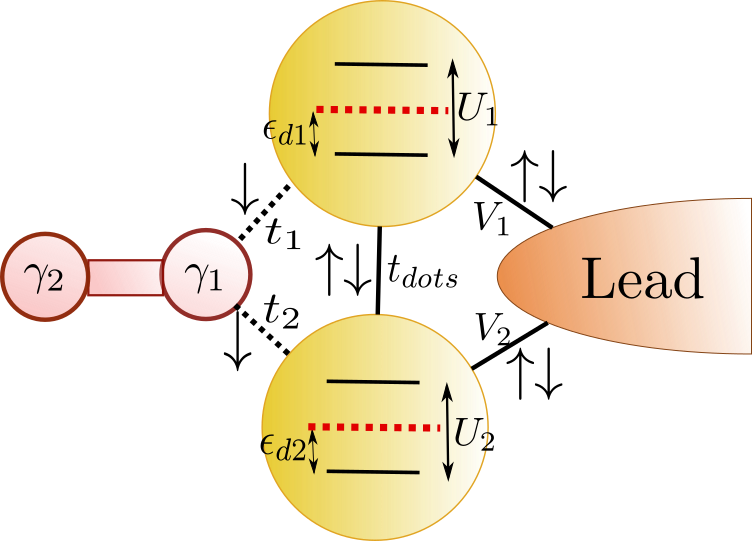
\includegraphics[scale=0.4]{IMAGES/GenModel.png}
    \caption{\label{fig:GenModel} Model for the DQD-Majorana system. Solid lines: Hopping interactions ($t_{dots}$: inter-dot coupling , $V_1,V_2$ couplings of QD1 and QD2 with the lead. ). Dashed lines: Majorana spin-$\dw$ effective couplings \eqref{eq:MajoranaCoupling} $t_1,t_2$. The atomic energy levels appear inside each QD $\ep_1, \ep_2$ are tuned by the gate voltages. The coulomb interaction is represented by $U_1,U_2$.  The red dashed horizontal lines represent the Fermi level. \protect \Source{ } } 
\end{figure}

\noindent The DQD-Majorana model is the most fundamental structure where Majorana manipulation is possible. Tunneling Majorana modes in this device have already inspired a few theoretical studies \cite{silva_andreev_2016,ivanov_coherent_2017} and experimental setups confirming the observations of Andreev molecules \cite{su_andreev_2017}. However, there is still no complete analysis of the transitions of the Majorana signatures between the QDs in this model, even though quantum tunneling of a MZM into a double dot offers several possibilities for MZM manipulation.  

 In this chapter, we will explore  different possibilities for Majorana manipulation in a device consisting of a DQD coupled to a MZM and a metallic lead (See \ \ref{fig:GenModel}). The simplicity of this model allows us to explore analytically different geometries of QD's from linear and symetric couplings to T-junctions (Fig.\ \ref{fig:MajoranaModels}). As in the previous models , we will consider both non-interacting and interacting regimes. 


% Tunneling of a MZM into a double dot shows several possibilities for manipulation of MZM,  there is still no complete analysis of the transitions of the Majorana signatures between the QDs in this model. 


% \noindent The idea of using Majorana islands formed by QDs coupled to topological superconducting wires has recently turned on new lights  into the fabrication of of quantum architectures \cite{barkeshli_physical_2015,karzig_scalable_2017}. The main insight  of this method is that today’s precise experimental control over the parameters of QDs -energy levels, tunneling couplings, etc.- offers the unique possibility of manipulating the Majorana modes inside multi-dot systems. The simplest case where Majorana manipulation is possible is in a double quantum dot. So far, no complete analysis of this basis case has been done. The purpose of this chapter is to fill this gap by realizing a full quantum transport study of the effects of coupling a Majorana mode with a double quantum dot. For this, we combine the ballistic transport and the NRG approach developed in \ref{chap: Methods}. 


% As previously stated in the , Majorana-QD  architectures turn on new lights to the area of topological quantum computing. 



% Using the ideas from the previous chapters we are going to test if it is possible to manipulate the Majorana zero mode in the double quantum dot.  

% In the previous chapter we observed the result of coupling a Majorana mode to a quantum dot. The Majorana signature characterized by a decay of the Fermi peak to the half of its original height is a



 The model in \ref{fig:GenModel} can be described from the combination of the Hamiltonians of a QD-Majorana system \eqref{eq:QD-Mham} and a DQD \eqref{eq:HDQD}. Integrating these models we obtain

\begin{equation}
H =\sum_{i=1}^2\sum_{k,\sigma}\left(\epsilon_{i}+\frac{U_i}{2}\right)d_{i\sigma}^{\dagger}d_{i\sigma}+ \frac{U_i}{2}(d_{i \sigma}^{\dagger}d_{i \sigma}-1)^{2} + t_i(\gamma d_{i,\dw}+d^\dagger_{i,\dw}\gamma) + V_id^\dagger_{i\sigma}c_{k\sigma}+V_i^* c^\dagger_{k\sigma}d_{i\sigma}.
\label{eq:Generalmodel}
\end{equation}

Where $V_1,V_2$ is the coupling of dots $1,2$ to the lead. $t_1,t_2$ define the Majorana couplings with each dot. $t_{dots}$ is the interdot coupling. $\ep_1,\ep_2$ are the energy levels of the dot, which are tuned by the the gate voltage and $U_1,U_2$ are the coulomb repulsion parameters. 
% \Jesus{I neglected $\epsilon_M$ in this case. Depending on the future NRG results I will choose to add it or leave it that way. }



\section{Applying our methods to the DQD-Majorana system}


% In order to understand the physical properties of this model, we probed a set of thought processes. The main variable in this analysis is the density of states.  We  will observe its evolution on both QDs under the tuning of the model parameters such as the majorana couplings ($t_1 , t_2$)  ,  gate voltages ($\ed{1} , \ed{2} $) and the inter dot coupling ($t_{dots}$). With these processes intend to show whether it is possible to "manipulate" the majorana modes inside the dots by tuning the established parameters. The number of possible combinations of parameters is huge and not all of them lead to important results. So on, we used the ballistic transport to select which arrangements could bring novel results. The most interesting models were simulated with NRG in the interacting case \ref{fig:MajoranaModels}.  

\subsection{Non-interacting Green function:}

%  To solve the transport equations using the graph method from \ref{sec:GraphMethod} first not that 
This new model is a combination between the DQD  (\ref{fig:graphDQD}) and the Majorana-QD  \ref{fig:green-M-QD}(b). We can use the trick in \ref{sec:GreenMaj-DQD} to get rid of the Green function $\Green{f_\dw,d^\dagger_1}$ for the second Majorana operator. This allows us to obtain the following transport equations 
 
 
 
%  As we did previously in \ref{sec:GreenMaj-DQD} the transport equations for $f_\dw$ and $f^\dagger_\dw$ are 
% \begin{align}
%         \left(\omega-\epsilon_{M}\right)\Green{f_{\downarrow},d_{1\downarrow}^{\dagger}}&=\frac{t}{\sqrt{2}}\left(\Green{d_{1\downarrow},d_{1\downarrow}^{\dagger}}-\Green{d_{1\downarrow}^{\dagger},d_{1\downarrow}^{\dagger}}\right) \\
%     \left(\omega+\epsilon_{M}\right)\Green{f_{\downarrow}^{\dagger},d_{1\downarrow}^{\dagger}}&=\frac{t}{\sqrt{2}}\left(\Green{d_{1\downarrow},d_{1\downarrow}^{\dagger}}-\Green{d_{1\downarrow}^{\dagger},d_{1\downarrow}^{\dagger}}\right),
% \end{align}
% \noindent which allows us to take $\Green{f_{\downarrow}^{\dagger},d_{1\downarrow}^{\dagger}} = \frac{\omega + \epsilon}{\omega -\epsilon}\Green{f_{\downarrow}^{\dagger},d_{1\downarrow}^{\dagger}} $. Therefore, we can eliminate $\Green{f_{\downarrow}^{\dagger},d_{1\downarrow}^{\dagger}} $ from the equations even before we start Gauss-Jordan process.
 
 \begin{equation}
     \left[\begin{array}{ccccccc}
\omega-\epsilon_{1} & -V_{1}^{*} & -t_{dots} & -T_{1} & 0 & 0 & 0\\
-V_{1} & \omega-\epsilon_{k} & -V_{2} & 0 & 0 & 0 & 0\\
-t_{dots}^{*} & -V_{2}^{*} & \omega-\epsilon_{2} & -T_{2} & 0 & 0 & 0\\
-T_{1}^{*} & 0 & -T_{2}^{*} & \omega-\epsilon_{M} & T_{2}^{*} & 0 & -T_{1}\\
0 & 0 & 0 & T_{2} & \omega+\epsilon_{2} & V_{2}^{*} & t_{dots}^{*}\\
0 & 0 & 0 & 0 & V_{2} & \omega+\epsilon_{k} & V_{1}\\
0 & 0 & 0 & T_{1} & t_{dots} & V_{1}^{*} & \omega+\epsilon_{1}
\end{array}\right]\left[\begin{array}{c}
\Green{d_{\mathbf{1\downarrow}},d_{1\downarrow}^{\dagger}}\\
\Green{c_{k\downarrow},d_{1\downarrow}^{\dagger}}\\
\Green{d_{2\downarrow},d_{1\downarrow}^{\dagger}}\\
\Green{f_{\downarrow},d_{1\downarrow}^{\dagger}}\\
\Green{d_{2\downarrow}^{\dagger},d_{1\downarrow}^{\dagger}}\\
\Green{c_{k\downarrow}^{\dagger},d_{1\downarrow}^{\dagger}}\\
\Green{d_{1\downarrow}^{\dagger},d_{1\downarrow}^{\dagger}}
\end{array}\right]=\left[\begin{array}{c}
0\\
0\\
0\\
0\\
0\\
0\\
1
\end{array}\right],
 \end{equation}
 
 where $T_i = \frac{t_i}{\sqrt{\omega+\epsilon_M}}$. 
 
 
% ------------------------FIGURE GRAPH--------------------
     \begin{figure}[bt]
    \centering
    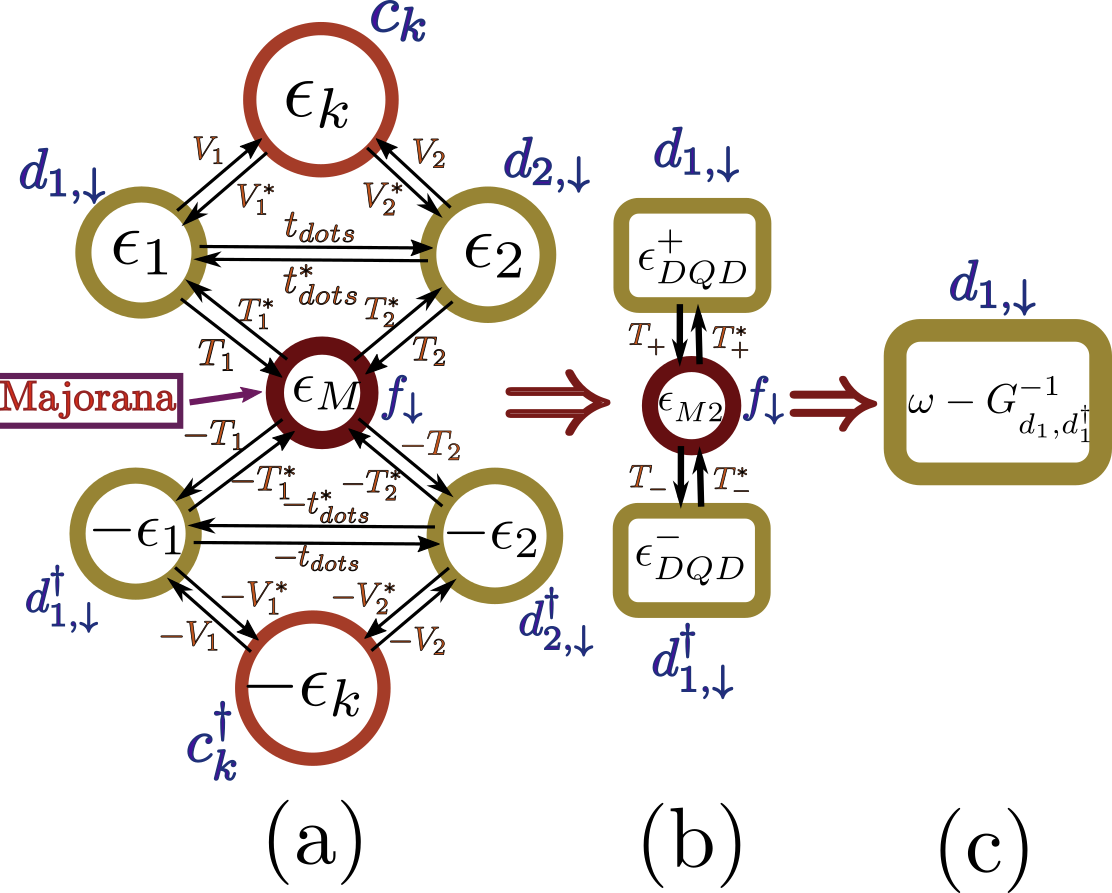
\includegraphics[scale=0.4]{IMAGES/Graphs/FinalGraph.png}
    \caption{\label{fig:Graph-MDQD} Graph method applied to a DQD coupled to a Majorana zero mode. a) Initial stage. b) Eliminated vertexes $c^\dagger_k$, $c_k$, $d_{2, \downarrow}$ , $d^\dagger_{2, \downarrow}$ in that order. c) Eliminated vertexes $d^\dagger_{1, \downarrow}$ and $f_\dw$, the final energy is $\omega-\Green{d_1,d_1^\dagger}$  . \protect\Source{   }} 
    \end{figure}

% ------------------------FIGURE GRAPH---------------------------
 The graph representing this equation is in  \ref{fig:Graph-MDQD}(a). Using the algorithm in \ref{sec:Algorithm} we start eliminating vertexes $c_k,c^\dagger_k, d_{2,\dw}$ and $ d^\dagger_{2,\dw}$ in that order. The self-energies associated to $d_{1,\dw}$ and $d^\dagger_{1,\dw}$ will be similar to the energy of the DQD \eqref{eq:EnDQD} giving 
\begin{equation}
    \epsilon_{DQD}^{\pm}=\pm\epsilon_{1}+\sum_{\mathbf{k}}\frac{V_{1}V_{1}^{*}}{\omega-\epsilon_{\mathbf{k}}}+\frac{\left\Vert \pm t_{dots}+\sum_{\mathbf{k}}\frac{V_{1}V_{2}^{*}}{\omega-\epsilon_{\mathbf{k}}}\right\Vert ^{2}}{\omega\pm\epsilon_{2}-\sum_{\mathbf{k}}\frac{V_{2}V_{2}^{*}}{\omega-\epsilon_{\mathbf{k}}}}. \label{eq:epDQD}
\end{equation}
\noindent There is also a correction in the couplings between the Majorana mode and $d_{1,\dw}$, $d^\dagger_{1,\dw}$ given by 

\begin{equation}
    T_{\pm}=\pm t_{1}\pm t_{2}\frac{\left(\pm t_{dots}+\sum_{\mathbf{k}}\frac{V_{1}V_{2}^{*}}{\omega-\epsilon_{\mathbf{k}}}\right)}{\omega\pm\epsilon_{2}\pm\sum_{\mathbf{k}}\frac{V_{2}V_{2}^{*}}{\omega-\epsilon_{\mathbf{k}}}}. \label{eq:T+-}
\end{equation}

\noindent In addition, since the Majorana is in contact with dot $2$, there is an extra-term appearing in the  Majorana self-energy given by 
\begin{equation}
    \epsilon_{M2}=\omega-\epsilon_{M}-\frac{\frac{\omega}{\omega+\epsilon_{M}}\left\Vert t_{2}\right\Vert ^{2} } {\omega-\epsilon_{2}-\sum_{\mathbf{k}}\frac{V_{2}V_{2}^{*}}{\omega-\epsilon_{\mathbf{k}}}}-\frac{\frac{\omega}{\omega+\epsilon_{M}}\left\Vert t_{2}\right\Vert ^{2}}{\omega+\epsilon_{2}-\sum_{\mathbf{k}}\frac{V_{2}V_{2}^{*}}{\omega+\epsilon_{\mathbf{k}}}}. \label{eq:M2}
\end{equation}
It only remains to eliminate out vertexes $d^\dagger_1$ and $f_\dw$  to obtain the green function 

\begin{equation}
    G_{{d_{1\downarrow},d_{1\downarrow}^{\dagger}}}\left(\omega\right)=\frac{1}{\omega-\epsilon_{DQD}^{+}-\frac{\left\Vert T_{+}\right\Vert ^{2}}{\omega-\epsilon_{M2}-\frac{\left\Vert T_{-}\right\Vert ^{2}}{\epsilon_{DQD}^{-}}}}.
    \label{eq:Green_NonInteracting}
\end{equation}

This simple formula summarizes the transport information through the first dot of the non-interacting Majorana-DQD system.  To compute the DOS we just need to replace  $\sum \frac{V_iV^*_i}{\omega -\epsilon_k}= -i\Gamma_i$ as performed in \ref{sec:GraphMethod}. By plotting the final DOS in Mathematica we were able to observe the transitions of the Majorana mode under manipulation of the model parameters.  


\subsection{NRG for the interacting system}

The Numerical Renormalization Group (NRG) technique described in \ref{sec:The-Numerical-Renormaliztion} is the most successful methods to study interacting quantum impurity models. In this model, the impurity is described by the DQD attached to the MZM. In our code, we set a Coulomb repulsion factor of $U =17.3\Gamma_1$ in both dots and a cut-off energy of $D=2U=34.6\Gamma_1$. The spacing with other energy levels is assumed to be higher than $D$, such that only the two coulomb states are relevant for the system dynamics.  When  $\epsilon_i = \frac{U}{2}$ in both dots, the system is in the Particle-Hole-Symmetric region. At this point, each dot has an odd number of electrons, hence, at sufficiently low temperature the system will exhibit characteristic Kondo peaks at the Fermi energy \cite{wilson_renormalization_1975}. The coexistence of Kondo and Majorana zero modes is still a point of contention in the area that has never been studied in DQDs and one of the objectives of this part of the project.


% Observing how the Kondo-effect interacts with the Majorana signature in the double quantum dot is also an insight of this project. 


To  improve the efficiency of the code we used the symmetries of the system to maintain a block structure during NRG's iterative diagonalization process. This model preserves the spin-$\up$ particle number $\hat{N}_\up$ and the spin-$\dw$ parity $\hat{P}_\dw = \pm $ ($+$ even, $-$ odd). The spin-$\dw$ particle number is not preserved due to superconducting-type Majorana coupling  \eqref{eq:MajoranaCoupling} . The initial Hamiltonian is organized in blocks according to these symmetries. This block structure is preserved during the entire iteration process \cite{bulla_numerical_2008}. To compute the spectral functions, we use the density matrix renormalization group (DM-NRG) described in \ref{subsec:DM-NRG} in combination with the Z-trick method \cite{oliveira_generalized_1994}, which improves spectral resolution at high energies.


To initialize the model in \ref{fig:Code} we set $H_{-1}$ equal to 
\begin{equation}
H_{-1} =\sum_{i=1}^2\sum_{k,\sigma}\left(\epsilon_{i}+\frac{U_i}{2}\right)d_{i\sigma}^{\dagger}d_{i\sigma}+ \frac{U_i}{2}(d_{i \sigma}^{\dagger}d_{i \sigma}-1)^{2} + t_i(\gamma d_{i,\dw}+d^\dagger_{i,\dw}\gamma),
\label{eq:imp_Ham}
\end{equation} 
\noindent and wrote the Hamiltonian in the symmetry-block diagonal representation (see \ref{sec:Double-Dot-Majorana-Hamiltonian.}). We also include manually the Hamiltonian $H_0$ into the code (See \ref{fig:Code}) to guarantee that both quantum dots are coupled to the first site of the chain. After this, the code follows the standard NRG algorithm and prints the density matrices to initialize DM-NRG. The final result is the spectral density which contains sufficient physical information to study the MZM-DQD model. In the following section, we show how the density of states can be used to simulate the Manipulation process of an MZM inside the DQD. 




\section{Manipulation of Majorana zero modes}


\begin{figure}[bt]
\centering
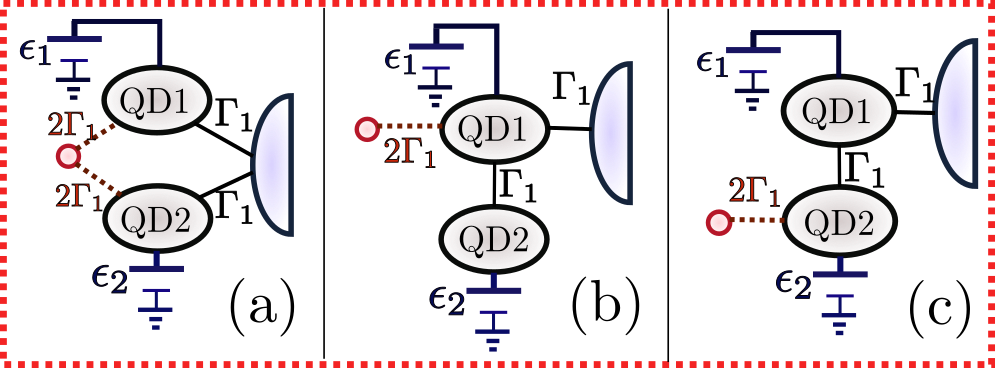
\includegraphics[scale=0.7]{IMAGES/DQD-M/3Model.png}
\caption{\label{fig:MajoranaModels}. \protect\Source{}} 
\end{figure}


The density of states provides significant information about the presence of a Majorana zero modes in the dot. We characterize the Majorana signature by a robust zero-mode with two possible heights:
 \begin{itemize}
         \item \textbf{Type I: }  The spin-$\dw$ DOS is the half of the spin-$\up$ DOS  at the Fermi energy $(\rho_\dw(0)=\rho_\up(0))$. 
         \item \textbf{Type II: } A spin-$\dw$ zero mode of height $ \rho_\dw(0) = \frac{0.5}{\pi  \Gamma_1}$. 
     \end{itemize}
In our results we observe several times these two types of signatures. Type I often appears when there is a zero-mode in the spin-$\up$ DOS, which is caused by the Kondo effect in the interacting case. Type II emerges in the remaining situations. 

We call MZM manipulation to the "movements" attributed to the Majorana signature under the tunning of the dot gate voltages $( \epsilon_1 , \epsilon_2 )$. This manipulation process is performed in three different set ups that are presented in \ref{fig:MajoranaModels} with definite values of $\Gamma_2$, $t_{dots}$, $t_1$ and $t_2$. In configuration (a), we coupled the QD symmetrically to the lead and the Majorana mode. With this setup we expect to break the localization of the MZM which should split and tunnel into both dots. In setups (b) and (c) we coupled the second dot indirectly through the first dot. Hence, quantum  interference should split the zero mode in two states. Our objective is to observe what occurs with the Majorana signature in this situation. There are two options to connect the MZM in this situation. Attached it directly through the first dot (b) or indirectly through the second dot (c). Both alternatives are geometrically distinct since (b) suggests a T-junction coupling while (c) reflects a connection  in series of both QD's between the lead and the MZM. 


 %-----------F I G U R E  t1 = t2 ------
\begin{figure}[H]
    \begin{center}
    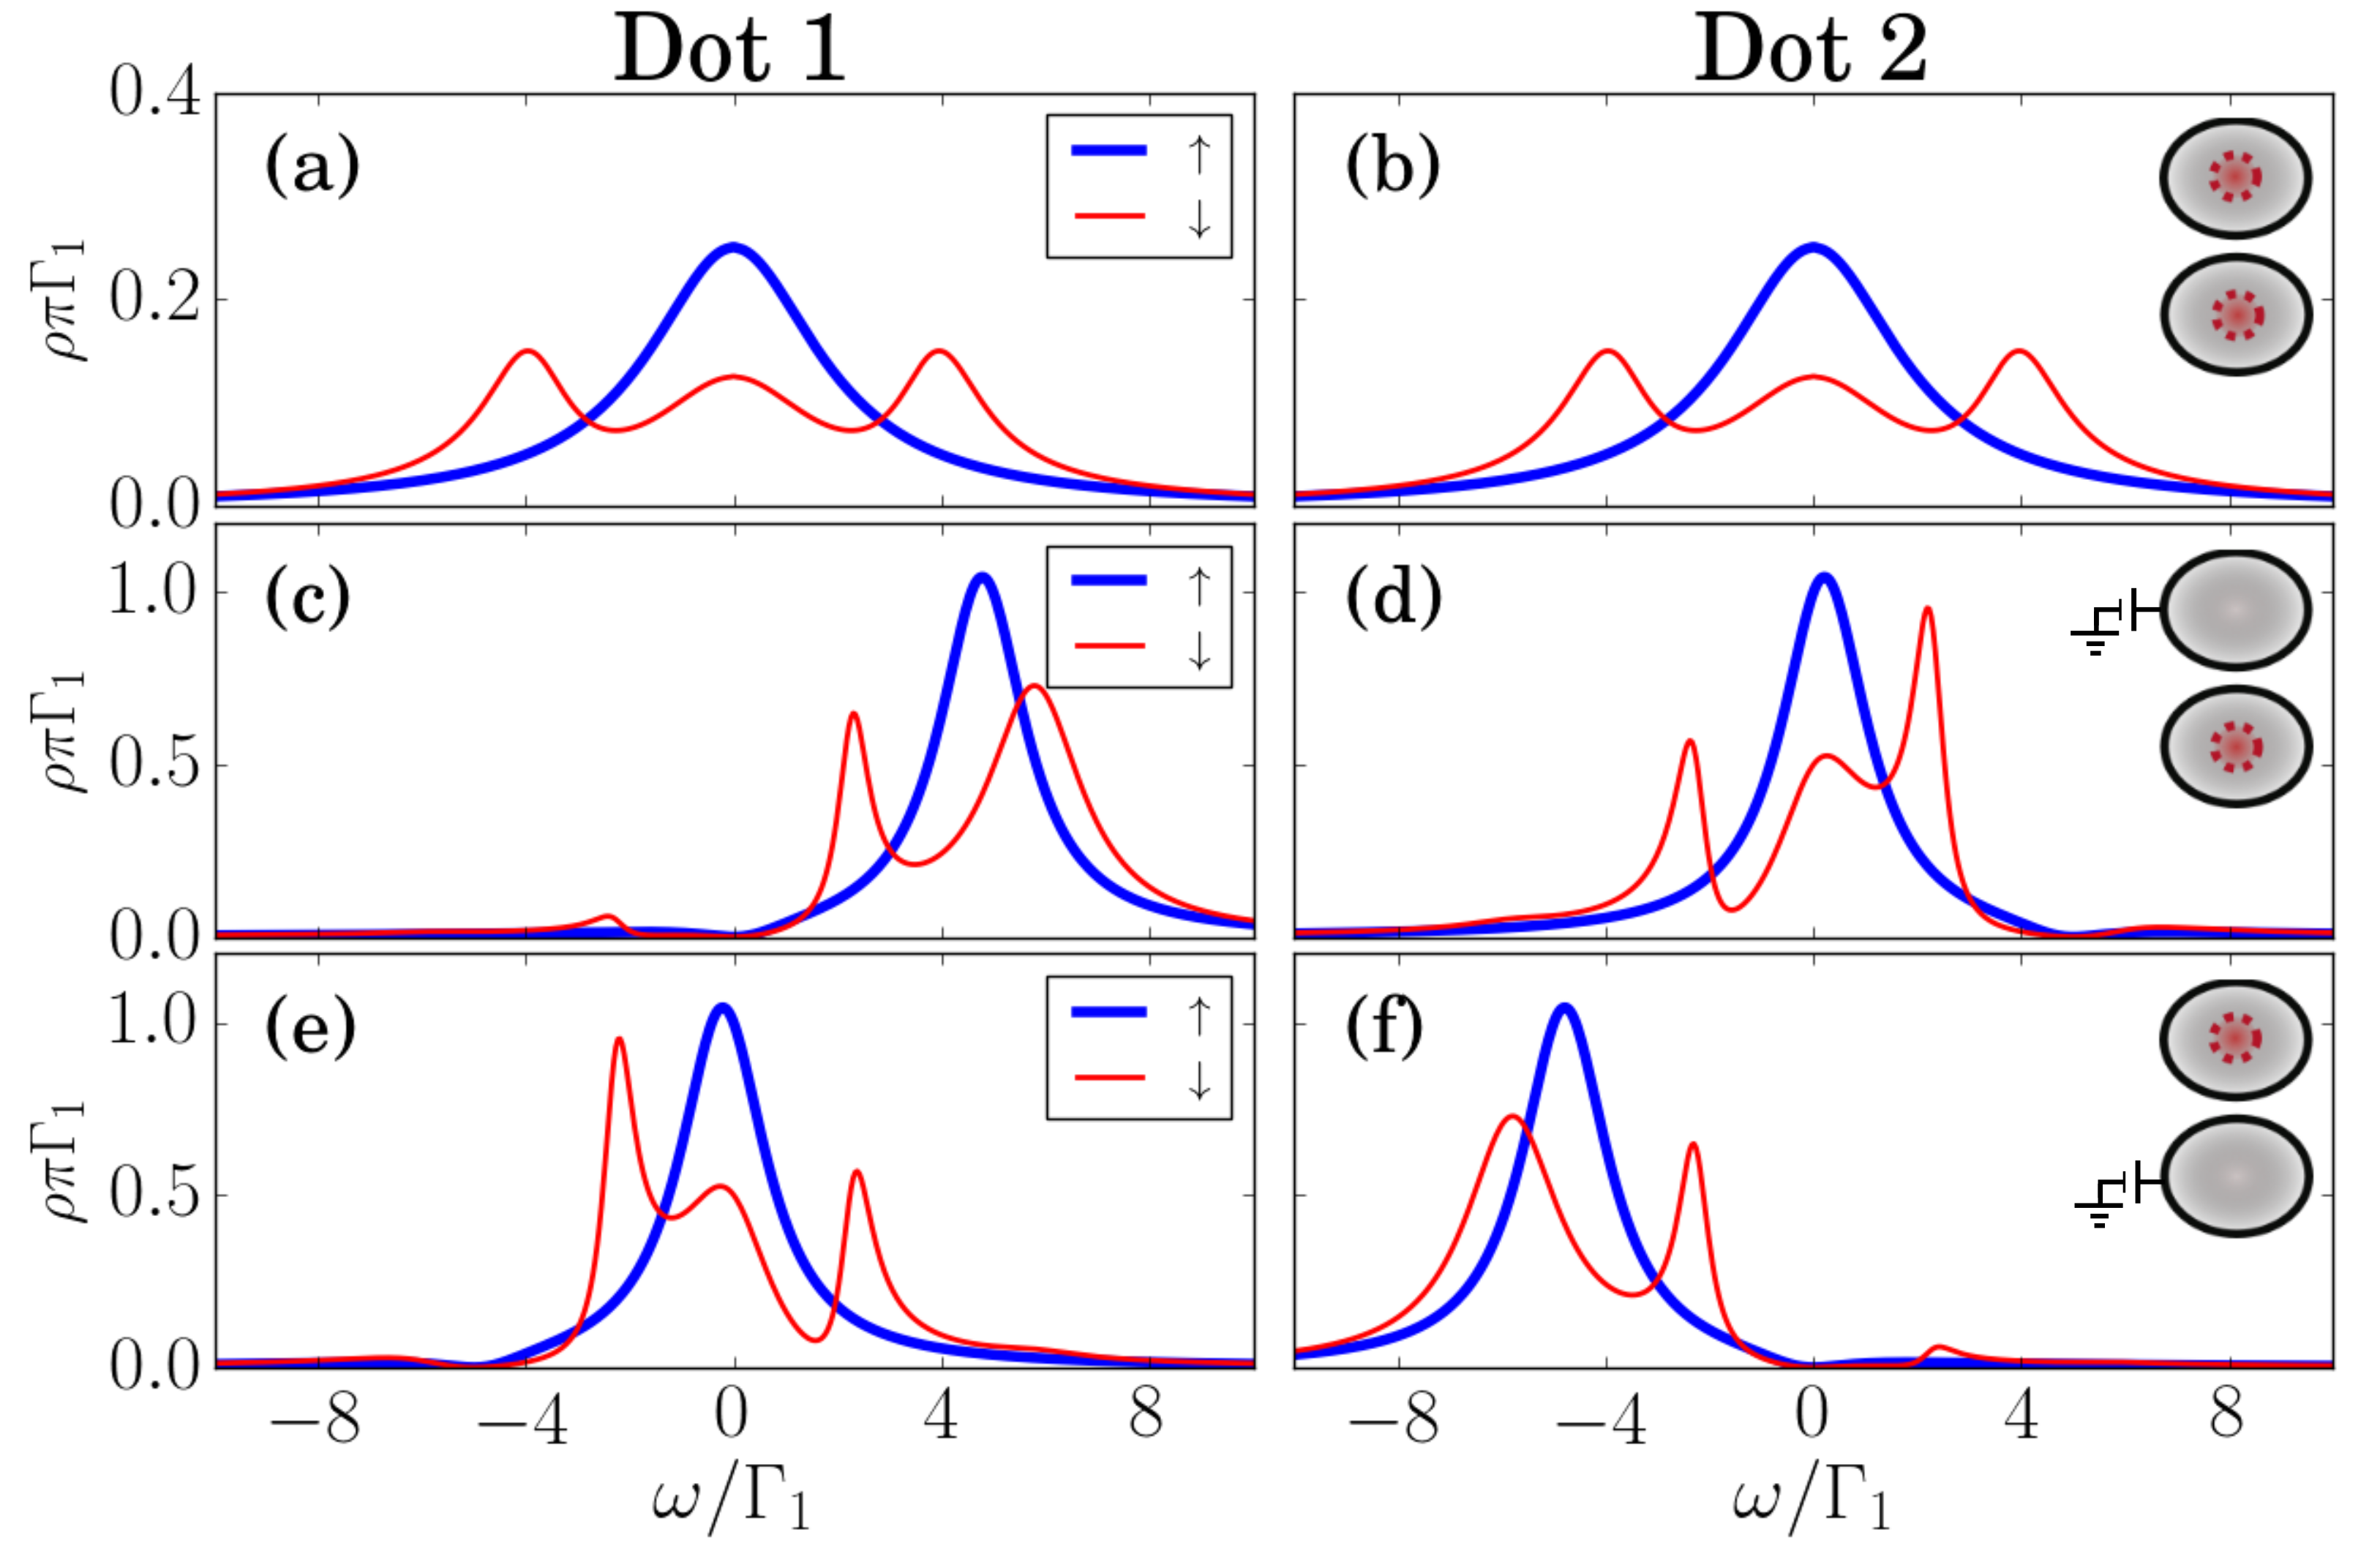
\includegraphics[scale=0.36]{IMAGES/GreenResults/t1=t2.png}
    \caption{ \label{fig:t1=t2}  Non-interacting DOS in the symmetric coupling(\ref{fig:MajoranaModels}(a)) at each QD. First column: Dot 1. Second column: Dot 2. The gate voltages vary at each row.  First row: Zero-bias in both dots $\ep_1=\ep_2=0$. Second row: $\ep_1=5\Gamma_1, \ \ep_2 =0$.  Third row: $\ep_1=0, \ \ep_2 =-5\Gamma_1$.  Bold blue lines: Spin-$\up$ DOS. Thin red lines: Spin-$\dw$ DOS. The insets at the right show which dot carries a Majorana signature, represented by a red dashed circle. Upper: First dot. Lower: Second dot. \protect\Source{}
    }
    %
    \end{center}
\end{figure}
%-----------F I G U R E  t1 = t2 ------

\subsection{Non-interacting manipulation}

 The non-interacting results for setups (a),(b) and (c) of \ref{fig:MajoranaModels} are shown at figures \ref{fig:t1=t2}, \ref{fig:t1>0} and \ref{fig:t2>0} respectively. Each figure depicts the DOS of dot $1$(left) and dot $2$(right). The gate voltage is initially $0$ in both dots at the first row. In the second row, the gate voltage is turned on to  $\epsilon_1 = 5\Gamma_1$ , while the second dot remains at $\epsilon_2 = 0$ . In the third row the first dot's voltage is off $\epsilon_1=0$ and we switch on the second dot with a negative voltage of $\epsilon_2 = -5\Gamma_1$. The inset figures at the right side of each row show which dots exhibit Majorana signatures, depicted by a red dashed circle inside the dot. These images will continuously change under the tuning of gate voltages which represents the manipulation of the Majorana signature.



In \ref{fig:t1=t2} we observe the results for the symmetric coupling setup \ref{fig:MajoranaModels}(a). In the particle hole symmetric case (first row) the DOS is equal in both dots. Note that the spin-$\dw$ (Thin red line) DOS is the half of the spin-$\up$ (Bold blue line) DOS at the Fermi energy $(\rho_\dw(0) = \frac{1}{2}\rho_\up(0))$. This type II Majorana signature is similar to the one observed when a single dot is coupled to a Majorana mode. \cite{liu_detecting_2011} We may conclude that the Majorana in tunneling inside both dots breaking the localization of the MZM. If a positive or negative gate voltage is induced in one of the dots, as shown in the second and third row of \ref{fig:t1=t2}(c)-(f),  the Majorana zero mode vanishes from that dot. Meanwhile the density of states in the other dot increases while preserving the Majorana signature. This means that the MZM is actually being induced to "leave" this dot and leak into the other by the biased voltage. This is the  first example of MZM manipulation. 


 %-----------F I G U R E  t1 >0 ------
\begin{figure}[bt]
    \begin{center}
    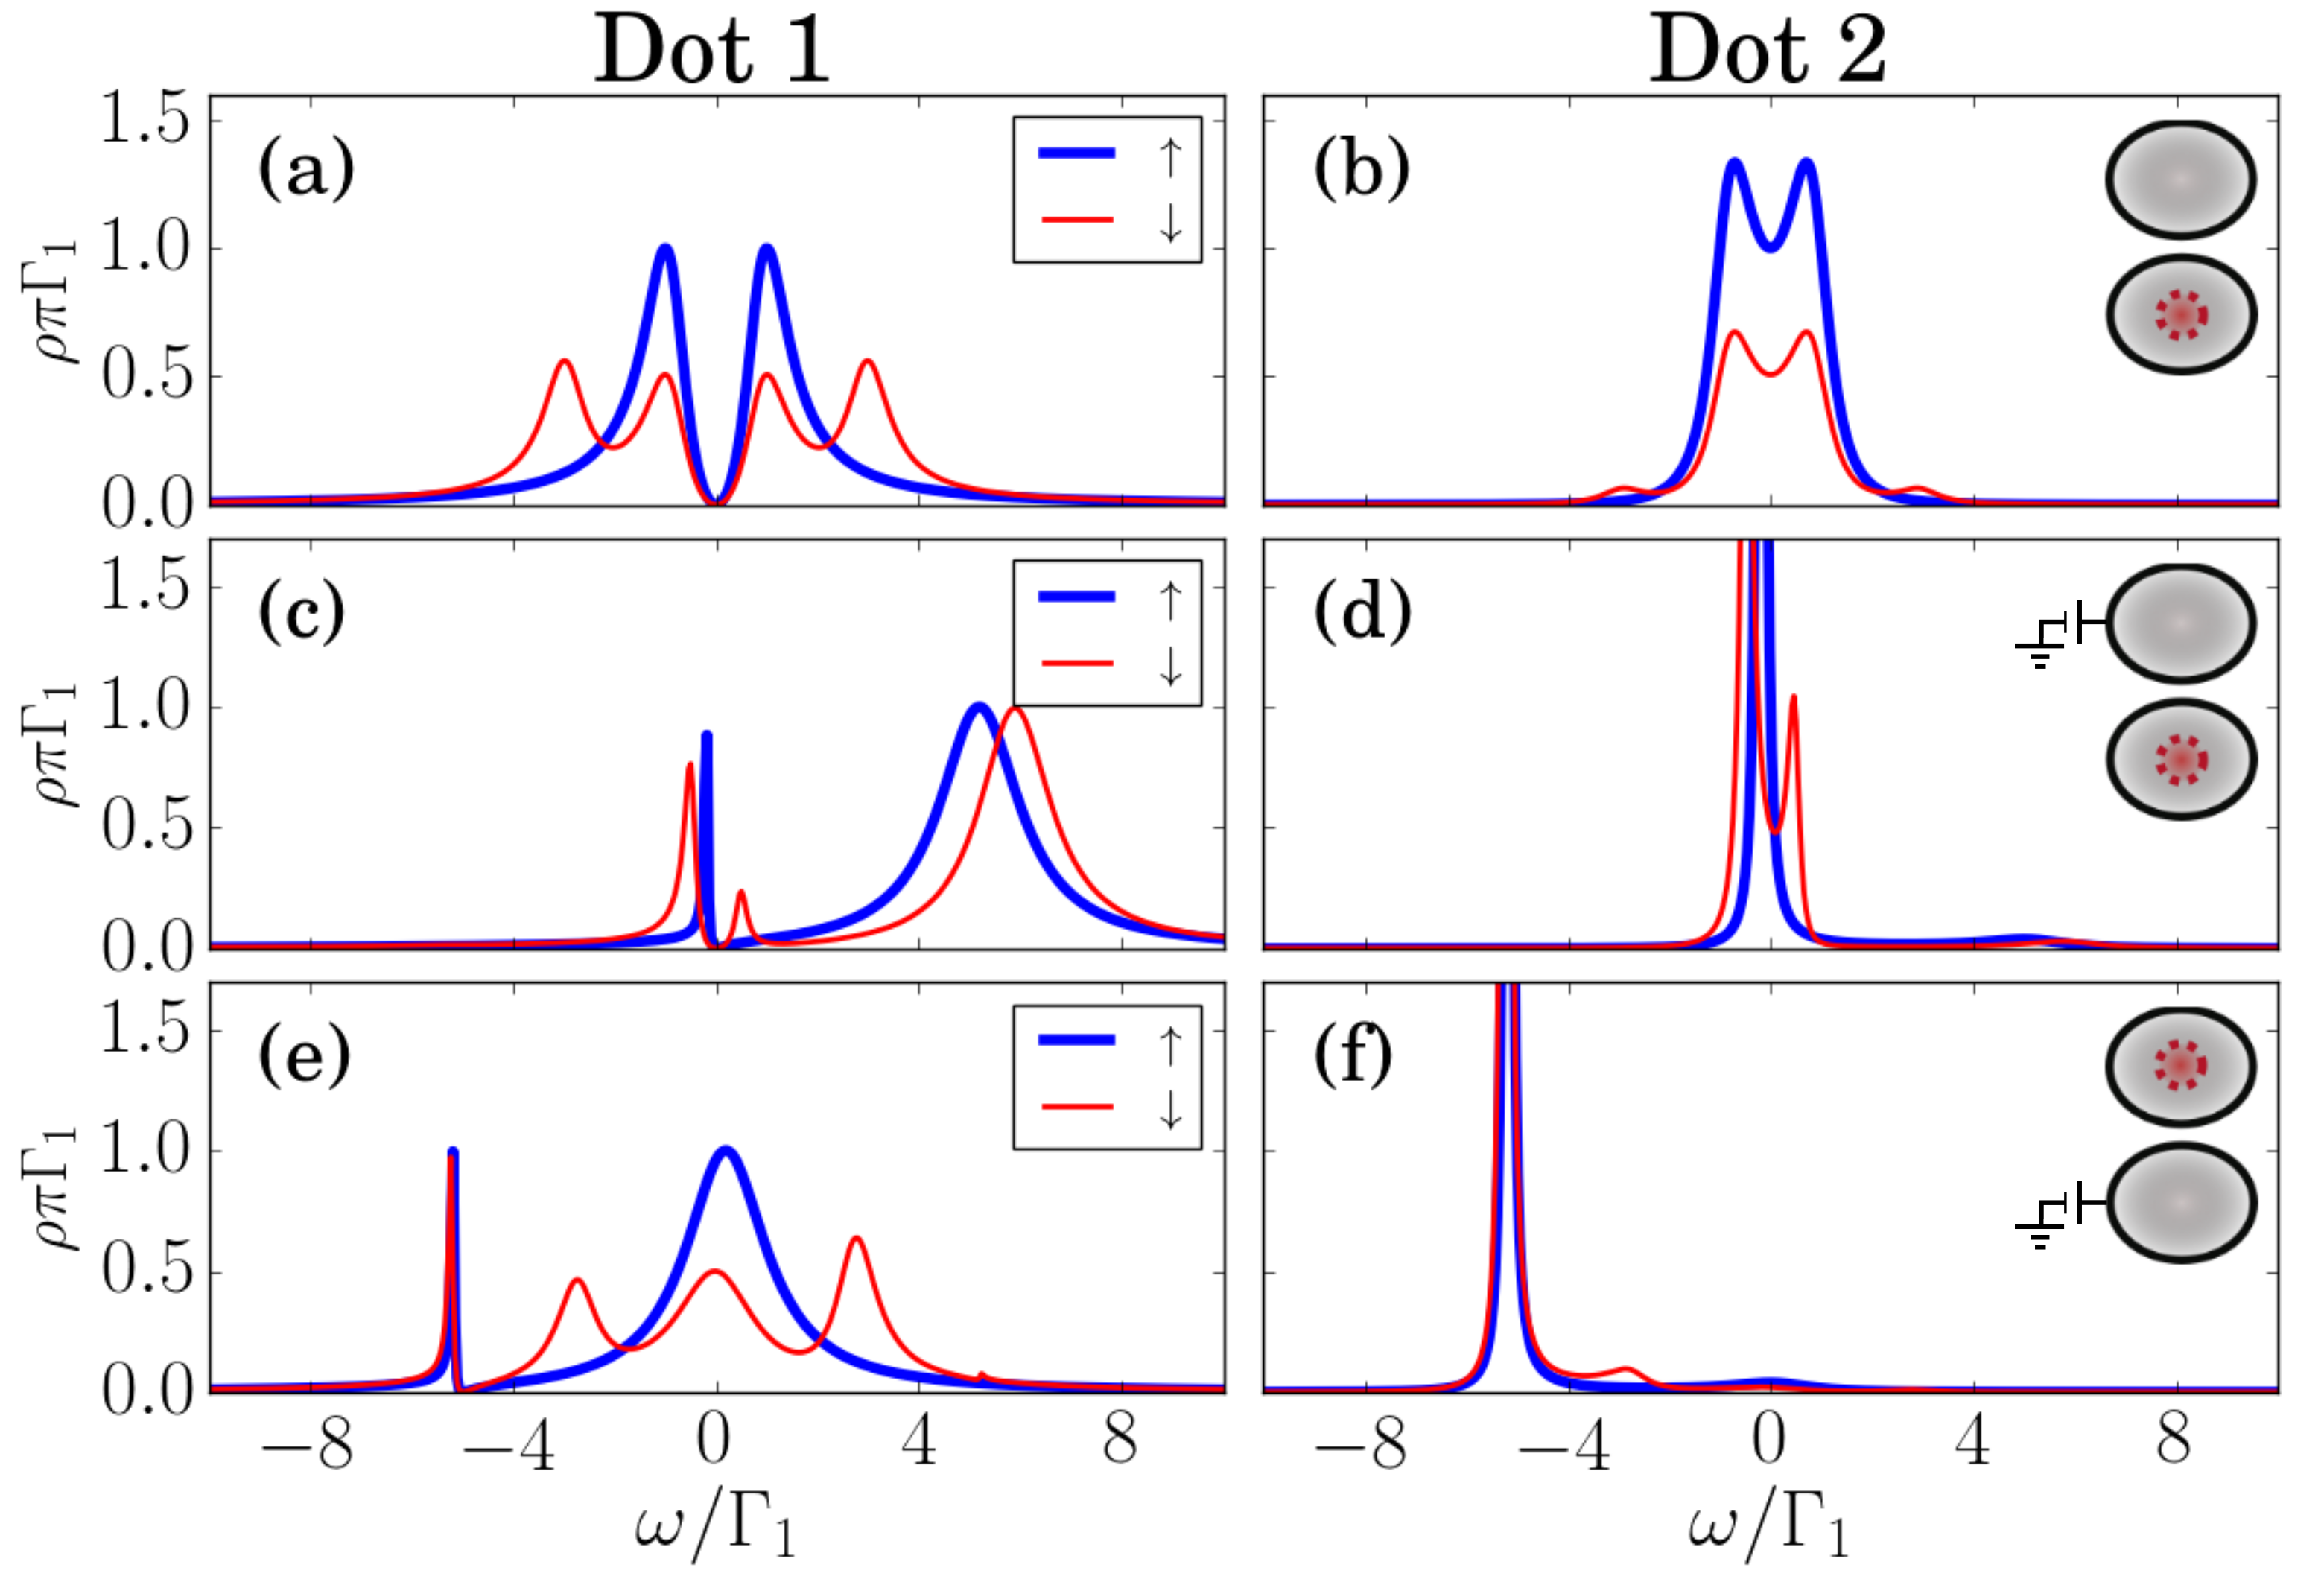
\includegraphics[scale=0.36]{IMAGES/GreenResults/t1>0.png}
    \caption{  \label{fig:t1>0} Non-interacting DOS of the T-dot coupling \ref{fig:MajoranaModels}(b). (b). First line (a),(b): $\ep_1=\ep_2=0$. Second line (c),(d): $\ep_1=5\Gamma_1$ , $\ep_2=0$. Third line (e),(f): $\ep_2=-5\Gamma_1$ , $\ep_1=0$.   Blue bold lines: Spin-$\up$ DOS. Red thin lines: Spin-$\dw$ DOS. The inset at the upper-right corner of each line indicates which dots  exhibit  Majorana signature, which is represented by a red dashed circle inside the dot. \protect\Source{}
    }
    %
    \end{center}
\end{figure}
%-----------F I G U R E  t1 >0 ------

Another example can  occur when the second dot is not directly connected to the lead. In this case, the inter-dot tunneling generates quantum interference which finally destroys the central peak as observed in \ref{fig:t1>0}(a) at the spin-$\up$ DOS . The spin-$\dw$ channel at \ref{fig:t1>0}(a), which is coupled to the MZM, does not exhibit the characteristic Fermi peak either. Instead, the one half Majorana signature at the Fermi energy $(\rho_\dw(0) = \frac{1}{2}\rho_\up(0))$ appears clearly inside the second dot \ref{fig:t1>0}(b). This situation prevails when the first dot's gate voltage is turned on \ref{fig:t1>0}(c)\&(d). While the first dot does not seem to exhibit any type of Majorana signature, the second dot's spin-$\dw$ DOS exhibits a robust zero-mode of height $\frac{0.5}{\pi \Gamma}$. The results are more exciting when the second dot's gate voltage is turned on in \ref{fig:t1>0}(e)\&(f). These figures clearly show how the MZM, previously localized at the second dot, is induced to leave this dot and to return into the first dot. Moreover, the DOS of spin-$\up$ and spin-$\dw$ channels are very similar to the spectral densities observed at \ref{fig:t1=t2}(d)(e), which means that the previous interference pattern has disappeared due to this gate voltage. 

 %-----------F I G U R E  t2 >0 ------
\begin{figure}[bt]
    \begin{center}
    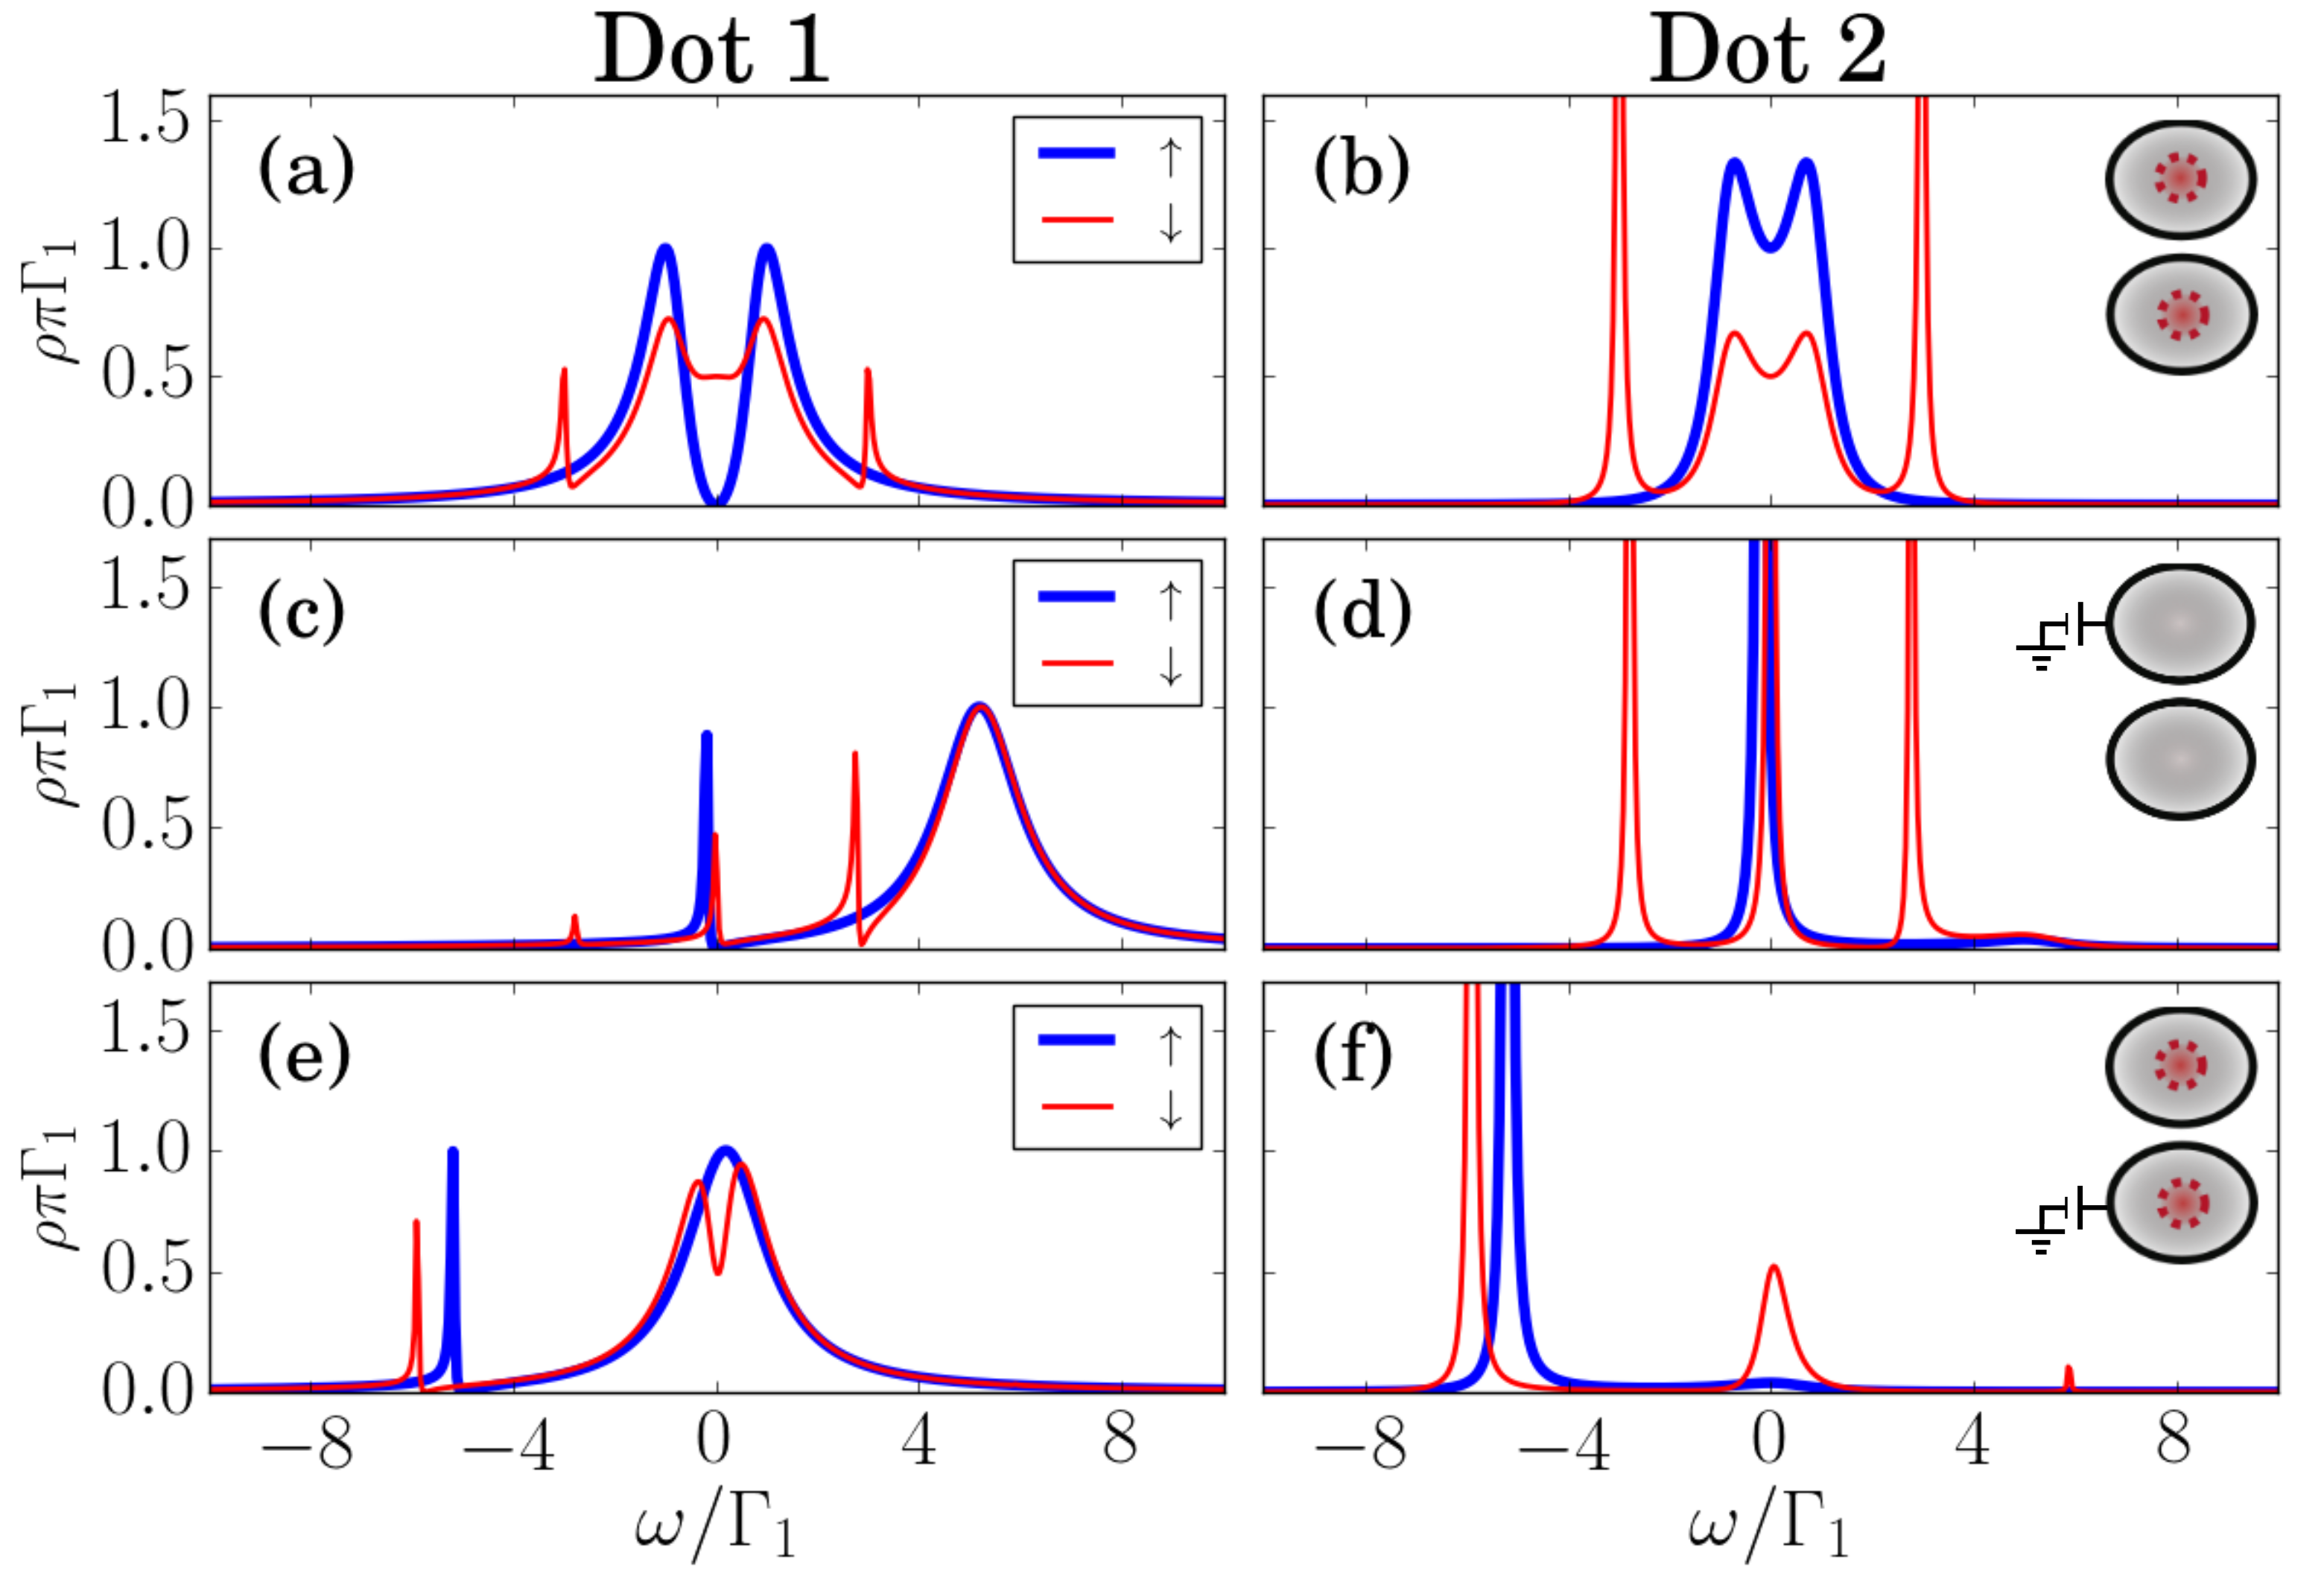
\includegraphics[scale=0.45]{IMAGES/GreenResults/t2>0.png}
    \caption{  \label{fig:t2>0}  Non-interacting DOS of the set up in \ref{fig:MajoranaModels}(c).  First line (a),(b): $\ep_1=\ep_2=0$. Second line (c),(d): $\ep_1=5\Gamma_1$ , $\ep_2=0$. Third line (e),(f): $\ep_2=-5\Gamma_1$ , $\ep_1=0$.   Blue bold lines: Spin-$\up$ DOS. Red thin lines: Spin-$\dw$ DOS. The inset at the upper-right corner of each line indicates which dots  exhibit  Majorana signature, which is represented by a red dashed circle inside the dot. \protect\Source{}
    }
    %
    
    \end{center}
\end{figure}
%-----------F I G U R E  t2 >0 ------


The results of the third configuration \ref{fig:MajoranaModels}(c) appear in \ref{fig:t2>0}. Contrary to what was observed in the previous case, this time the Majorana signature is not destroyed by the interference but instead, the  $\frac{0.5}{\pi \Gamma}$-height MZM emerges indirectly in the first dot. This is a perfect way to separate the Majorana's spin-$\dw$ DOS from the central spin-$\up$ zero-mode which is still destroyed by the interference. In addition, the second dot still exhibits a type I Majorana signature as observed in \ref{fig:t2>0}(b). In the second row we observe that turning on the gate voltage in dot $1$  destroys the Majorana signature in both dots \ref{fig:t2>0}(c)(d). On the other hand, if the second dot's voltage is switched both dots will preserve their Majorana signature (QD1:type I, QD2: type II), while the spin-$\up$ quantum interference vanishes in the first dot.






% In this part we will discuss the three models in figure \ref{fig:Models} which are particularly interesting for the exotic behavior of their Majorana signature. The parameters $(t_1,t_2, t_dots)$ are fixed in these three models and we will take $\ep_1$ and $\ep_2$ as variables. The first model(a), represents a symmetric coupling of the DQD with the lead and the Majorana mode. In models (b) and (c) the second dot is indirectly coupled to the system through the first dot. As already analyzed in \ref{sec:GreedDQD}, the quantum interference generated by this coupling will destroy the central peak. The Majorana fermion can be either connected to the first dot (b) or to the second dot (c). The system will exhibit different Majorana signatures depending on which dot is connected to the Majorana zero mode.   



% On each case we observe three different situations. 
% \begin{itemize}
%     \item First Row: Zero bias. No gate $\ep_1 =\ep_2 = 0$.
%     \item Second Row: We turn on the first dot's gate voltage $\ep_1 = 5\Gamma_1, \ep_2 = 0$.
%     \item Third Row: We turn on the second dot's gate voltage $\ep_2 = -5\Gamma_1, \ep_1 = 0$.
% \end{itemize}

    

%     The density of states for the setup in \ref{fig:Models}.(a) is shown in Figure \ref{fig:SymCoupling}. Since the model is non-interacting, spin-$\up$ and spin-$\dw$ models are independent. The spin-$\dw$ DOS (dashed line) shows the effects caused by the Majorana zero-mode in comparison with the spin-$\up$  results (solid line). In the particle hole symmetric (first line) the DOS is equal in both dots. Note that that the spin-$\dw$ DOS is the half of the spin-$DOS$ at the fermi energy $\rho_\dw(0) = \rho_\up(0)$. This Majorana signature is similar to the one observed in the single dot case \cite{liu_detecting_2011}. We may conclude that the Majorana tunnels inside both dots. If a positive or negative gate voltage is induced in one of the dots, as shown in the second and third row of Figure \ref{fig:SymCoupling},  the Majorana zero mode vanishes. Looking to the other dot we can also observe that the Majorana signature in the other dot recovers the form observed in the single dot-Majorana model. Thus, by activating the gate voltage in one of the dots it is possible to induce the majorana mode to leave to the other dot.  

    
     
%     If the second dot is not directly connected to the lead the induced tunneling between both dots generates a path difference that destroys the central peak (See FIG\ref{fig:Interference} spin-$\up$ line). We can then proceed to connect the Majorana to each one of these dots. \ref{fig:Interference} shows the results of connecting the MZM to the first dot. Note that at zero-bias, quantum interference  destroys the Majorana mode in the first dot. However, in the second dot the spin-$\dw$ DOS is the half of the spin-$\up$ DOS at the Fermi energy, which is a clear Majorana signature. Hence, in this kind of arrangement the Majorana mode is allocated in the second dot.  \ref{fig:Interference}(e),(f) show that it is possible to reestablish the initial Majorana signature in the first dot by applying a gate voltage to the second dot. On the other hand, turning on the first dot's gate voltage does not lead to a meaningful change in the Majorana signature \ref{fig:Interference}(c),(d). While the spin-$\dw$ DOS in the first dot is still $0$ at the Fermi energy, the second dot shows a $0.5$-height zero mode. Although the spin-$\up$ DOS does not double the density of states any more, this signal is robust and equal in height to a Majorana signature which supports our claim that it is indeed a Majorana mode. 
%     If the Majorana mode is connected to the first dot, this interference will destroy the Majorana signature in the first dot. Interestingly, it is possible to observe a clear Majorana signature in the second dot characterized by a half central peak in the spin-$dw$ DOS. While turning on the first dot gate voltage seems to destroy this Majorana signature, tuning the second dots gate voltage returns the Majorana signature to the first dot. 


%     We now get into the final case that is when the Majorana mode is coupled to the second dot which is indirectly attached to the lead through the first dot. In this case \ref{fig:IndirectCoupling}(a)(b) shows that the Majorana signature is present in both dots, despite the Majorana is not directly coupled to the first dot. Moreover, we can observe that the spin-$\dw$ DOS is equal to $0.5$ at the Fermi energy while the spin-$\up$ peak has been destroyed by the interference. After turning on the first gate voltage we observe that the Majorana signature is destroyed in both dots \ref{fig:IndirectCoupling}(c)(d). This is totally opposite the results of increasing the second dot voltage which creates an stable $0.5$ Majorana signature at the Fermi energy of both dots \ref{fig:IndirectCoupling}(e)(f). 






\subsection{Interacting manipulation \label{sec:DQD-M-Interacting}}

 %-----------F I G U R E  t1=t2 ------
\begin{figure}[bt]
    \begin{center}
    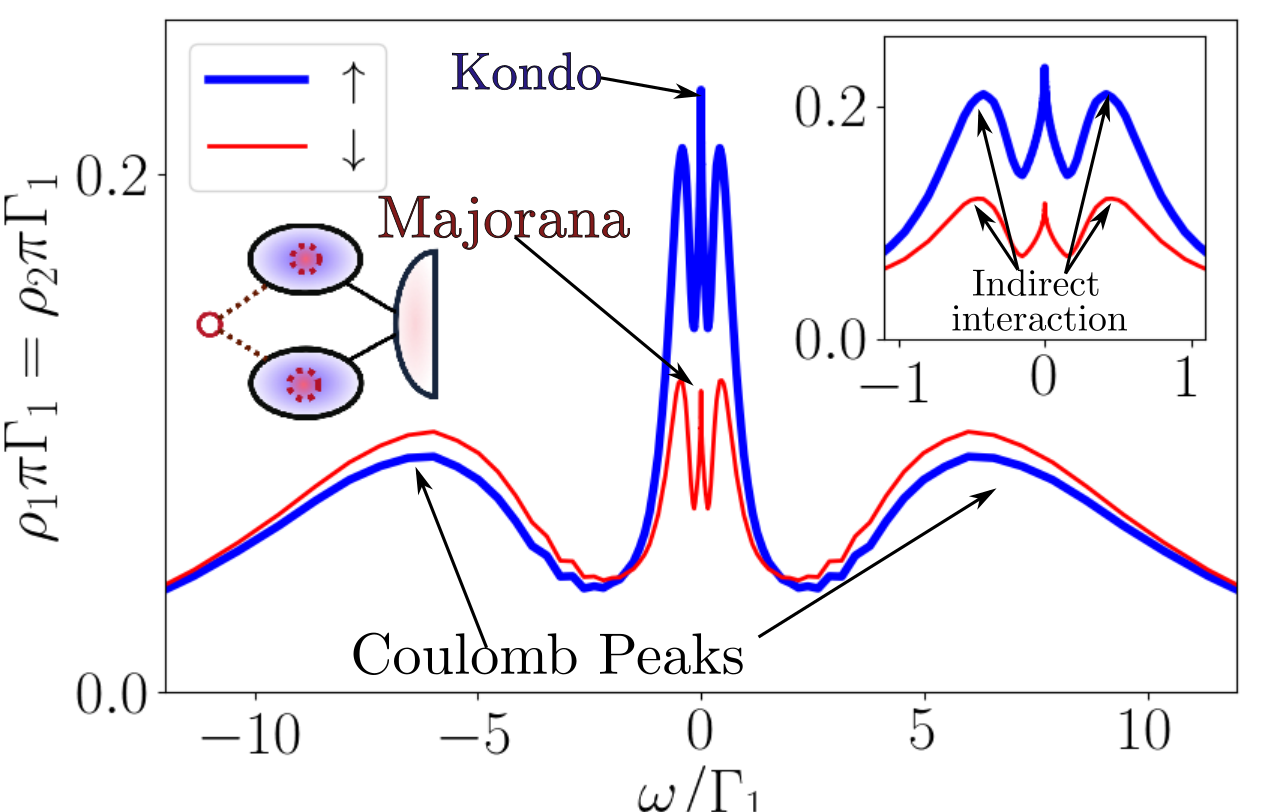
\includegraphics[scale=0.52]{IMAGES/NRG/NRG-t1=t2.png}
    \caption{  \label{fig:NRG_Majorana}    Density of states of both dots in the symmetric coupling without gate voltages between the Majorana and the interacting DQD. Bold blue lines: Spin-$\up$ DOS. Thin red lines: Spin-$\dw$ DOS. Inset: Low-energy DOS.\protect\Source{}
    }
    %
    \end{center}
\end{figure}
%-----------F I G U R E  t1 =t2 ------

Now we consider a Coulomb repulsion energy of $U = 17\Gamma_1$ in both dots. The factor $ \frac{U_i}{2}(\sum_{\sigma} \hat{n}_{i\sigma}-1)^{2}$ in \eqref{eq:Generalmodel} favors states with an odd number of electrons (and holes). In addition, particle-hole equilibrium is now achieved when $\Delta \epsilon_{i} := \left(\epsilon_{i}+\frac{U_i}{2}\right)$.  Any induced gate voltage must be considered as a shifting $\Delta \epsilon_{i}$ from this equilibrium point. \ref{fig:NRG_Majorana} shows the DOS of both QDs for the symmetric coupling configuration \ref{fig:MajoranaModels}. The two peaks appearing at around $8.6\Gamma_1 = \frac{U_i}{2}$ represent the two energy levels spaced by the Coulomb repulsion factor $U$. The central spin-$\up$ peak is a consequence of the Kondo effect, \cite{hewson_kondo_1997,wilson_renormalization_1975}  while the two satellite peaks observed in the inset  are the result of the  RKKY indirect interaction between both dots.  \cite{ruderman_indirect_1954,kasuya_theory_1956,yosida_magnetic_1957} Moreover, the system presents a Majorana signature characterized by half spin-$\dw$ DOS at the Fermi energy $(\rho_\dw(0) = \frac{1}{2}\rho_\up(0))$  . Note, that in this case the Majorana signature coexists with the Kondo effect in the DQD as already predicted by Ruiz-Tijerina \textit{et al.} for a single dot. \cite{ruiz-tijerina_interaction_2015}


% If the two dots are interacting, with $U = 17.6\Gamma_1$, the spin-$\up$ density of states for the symmetric configuration (\ref{fig:Models}.(a)) is pretty similar to the DQD-symmetric model. The height of the central peak decays to $0.25$ and two new peaks appear corresponding to the dots anti-ferromagnetic interaction. In the spin-$\dw$ channel we can observe a zero mode with height equal to the half of the spin-$\up$ DOS. The effect of the Majorana coupling can be observed better on \ref{fig:2D/Shift_t1=t2}. 

\begin{figure}[H]
    \centering
    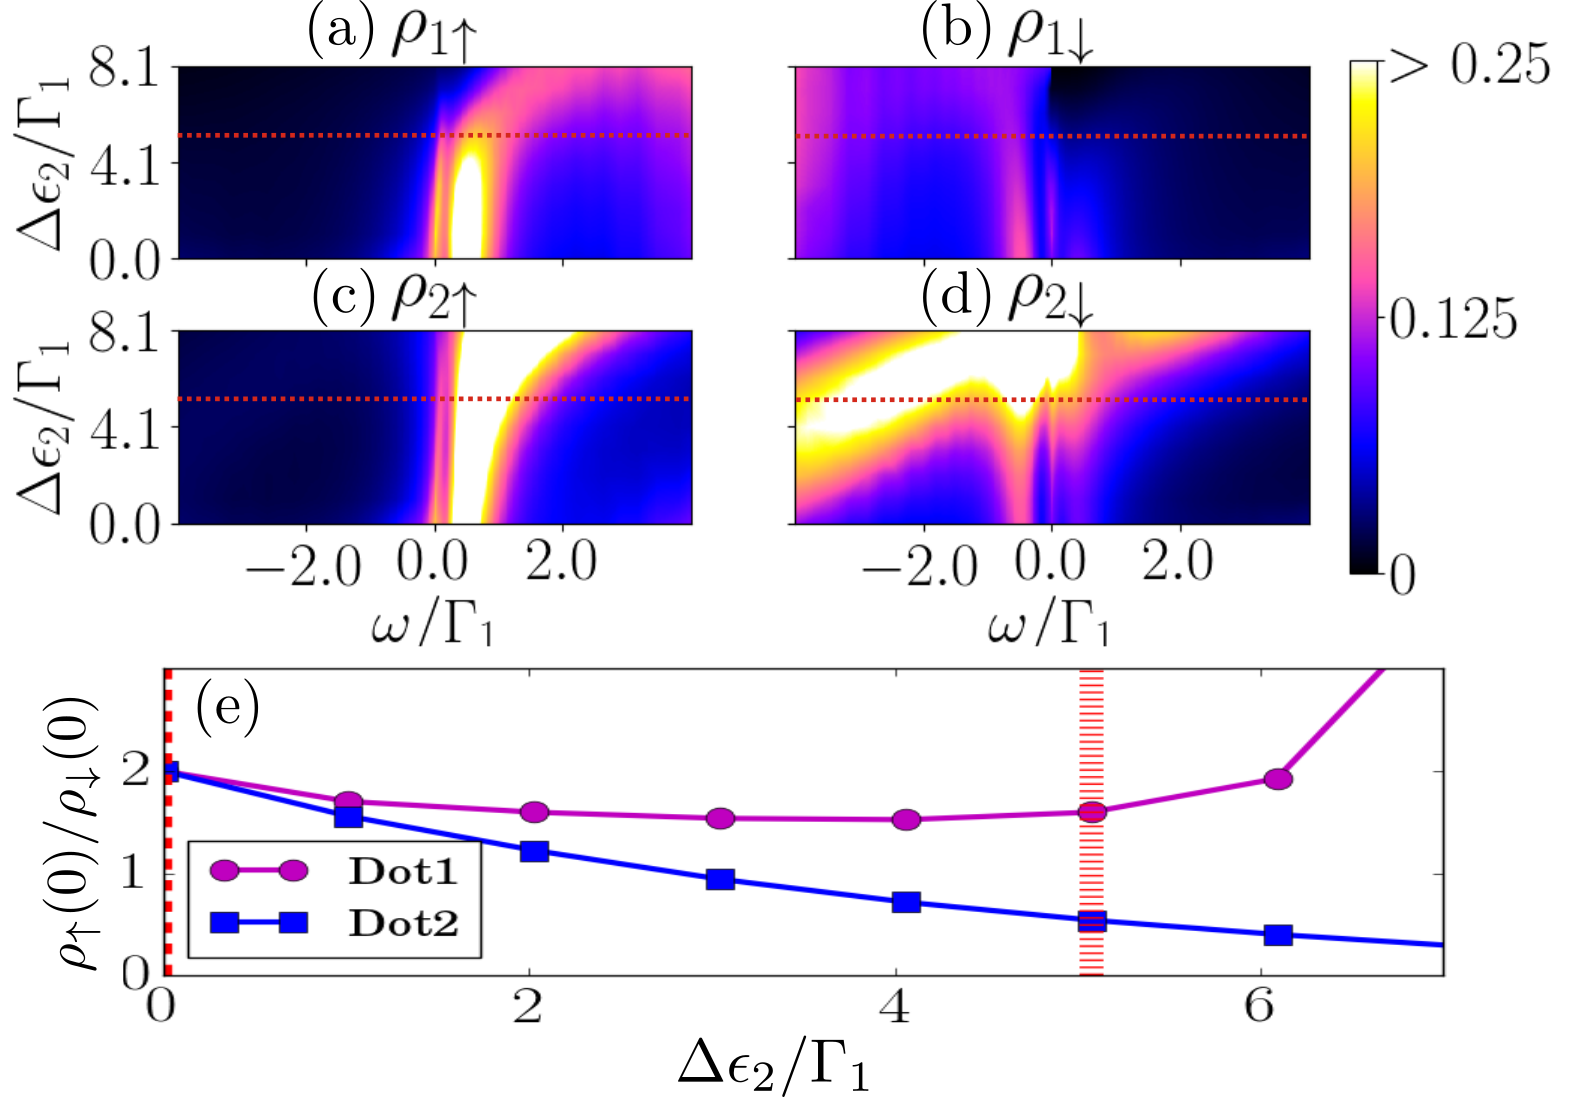
\includegraphics[scale=0.5]{IMAGES/NRG/FullEd2.png}
    \caption{\label{fig:ed2/Fermi} (a)-(d) Dependence of the density of states of setup in \ref{fig:MajoranaModels}(a) over $\omega$ and the gate voltage $\Delta \epsilon_2$ . $\Delta \epsilon_1=0$  Up: Dot 1. Down: Dot 2. Left: Spin-$\up$. Right: Spin-$\dw$.  (e) Evolution of the relation $\frac{\rho_\up(0)}{\rho_\up(0)}$ for both QDs. While QD2 losses rapidly the Majorana signature, QD1 maintains it till $\Delta \ed{2}\sim 5$. \protect\Source{}}
\end{figure}



    In this part of the project we are interested in the physics at low energy scales $\omega \sim \Gamma_1 $ close to the Kondo and MZM temperature. At this scale we can observe similar Majorana signatures compared with the non-interacting case. For instance, the inset \ref{fig:NRG_Majorana} shows the NRG results for the symmetric setup in \ref{fig:MajoranaModels}(a). In agreement with the non-interacting results, both dots have type I Majorana signatures. 

    When the gate voltage is turned on, we observe the number of holes $(\omega>0)$ increasing in the spin-$\up$, while the particles $(\omega<0)$ increase in the spin-$\dw$ (See \ref{fig:ed2/Fermi}(a)-(d) ). At $\Delta\epsilon_2 \approx 6\Gamma_1$, the Coulomb peak overlaps with the Fermi energy in the spin-$\downarrow$ channel, destroying the Majorana zero mode. This event is visible in \ref{fig:ed2/Fermi}(e), where the type one Majorana signature is clearly destroyed in Dot $1$ after $\Delta\epsilon_2 > 6\Gamma_1$. For $\Delta\epsilon_2 < 6\Gamma_1$ we observe an stable Majorana signature in dot $1$ with $\rho_\dw(0) \approx \frac{1}{2}\rho_\up(0))$. In the second dot the zero modes are absorbed by the dot, which slowly destroys the Majorana signature. 

     %-----------F I G U R E  7 ------
\begin{figure}[bt]
\begin{center}
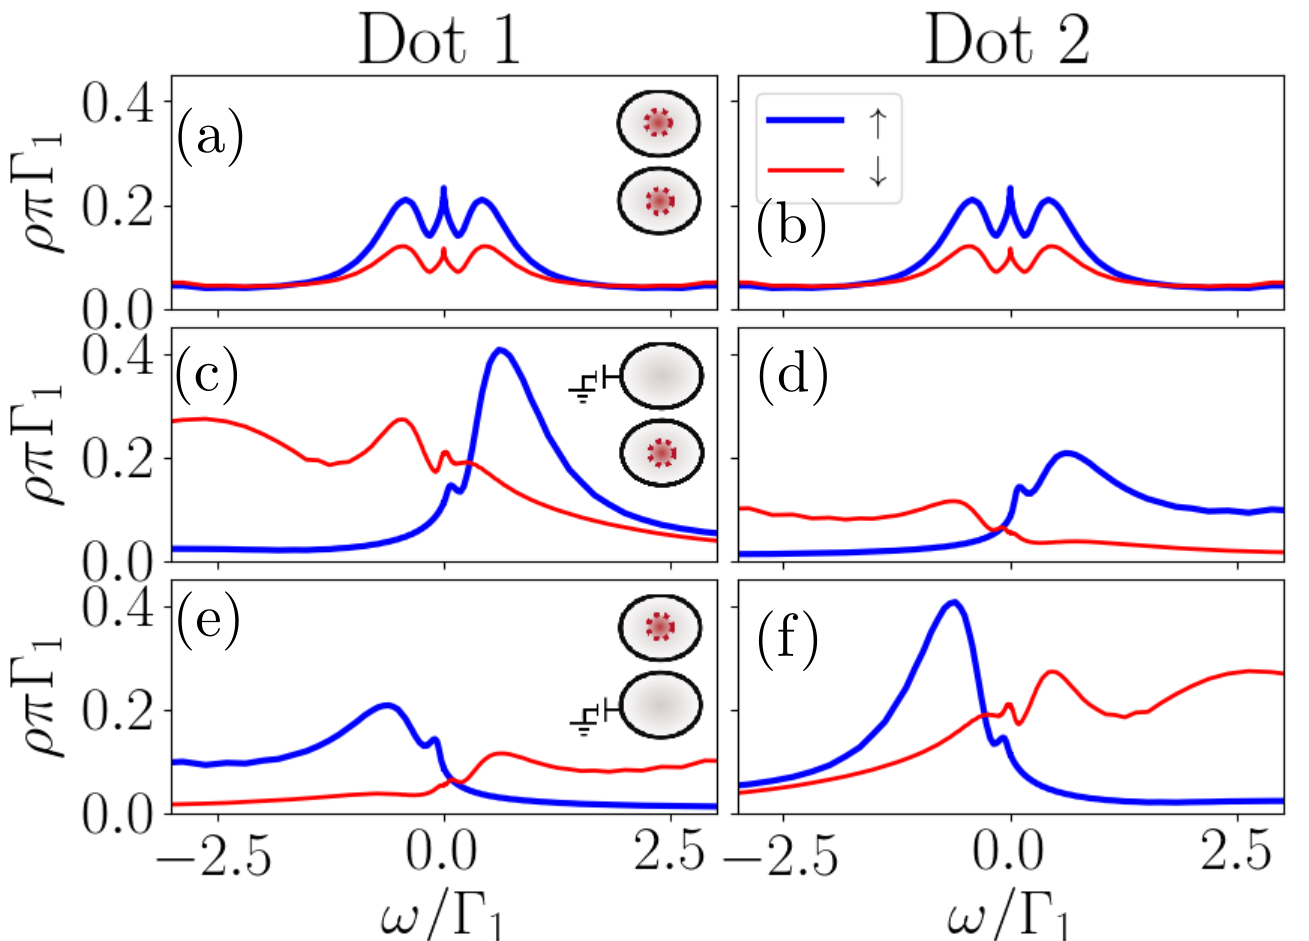
\includegraphics[scale=0.5]{IMAGES/NRG/t1=t2.png}
\caption{ \label{fig:Nt1=t2} The same as in \ref{fig:t1=t2} for the  interacting DOS in the symmetric coupling  (\ref{fig:MajoranaModels}.\protect\Source{}
}
%
\end{center}
\end{figure}
%-----------E N D  F I G U R E  7 ------

    The red cuts in \ref{fig:ed2/Fermi} are plotted in \ref{fig:Nt1=t2} where we depict the results of Majorana manipulation. In agreement with the non-interacting case, the particle hole symmetric model receives both Majorana modes. Whenever a gate voltage is switched on, the Majorana is forced to tunnel into the other dot. We observe similar results for positive and negative gate voltages. 

 
 In the T-dot coupling \ref{fig:MajoranaModels}(b), the spin-$\up$ Kondo peak in  \ref{fig:Nt1>0} is destroyed by interference just as in the non-interacting case. This phenomenon had already been predicted for a T-junction of a double quantum dot attached to metallic leads \cite{dias_da_silva_transmission_2008}. The insight of our model is that an attached MZM should also disappear due to the same interference. Furthermore, a type I Majorana signature can be observed at very low energies in the inset of \ref{fig:Nt1>0}(b). However we have to recognize that both zero-modes decay significantly in the second dot. When the first voltage is turned on, the Majorana mode jumps onto the first dot which presents a type I Majorana signature. This is a clear difference with the non-interacting results where the Majorana signature stayed in the second dot.  If the second dot is switched on , a type II Majorana signature appears at very low energies in dot 1, which is coherent with the idea that the Majorana interference should disappear in this case. In \ref{fig:Nt1>0}(e) we identify emergence of a Fano resonance at the Fermi energy causing the sharp-asymmetric peak at $\omega = 0$. Fano resonances have already been documented in similar models in \cite{schuray_fano_2017}. We are going to talk more about this resonance in following section. 



 %-----------F I G U R E  4 ------
\begin{figure}[bt]
\begin{center}
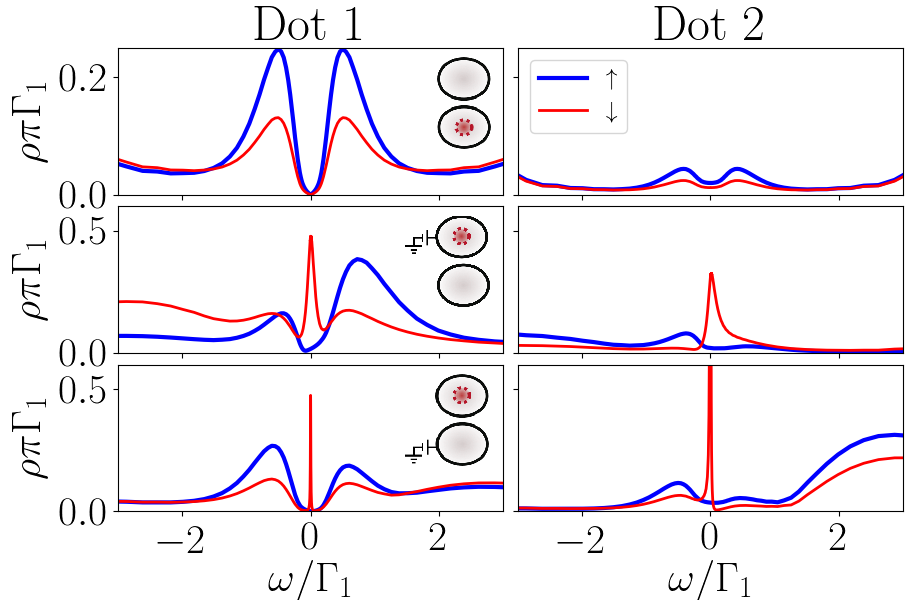
\includegraphics[scale=0.4]{IMAGES/NRG/t1>0.png}
\caption{  \label{fig:Nt1>0} The same as in \ref{fig:t1=t2} for the  interacting DOS of the T-dot junction \ref{fig:MajoranaModels}(b). Inset in b): Zoom to low-energy DOS. \protect\Source{}
}
%
\end{center}
\end{figure}

\begin{figure}[H]
    \centering
    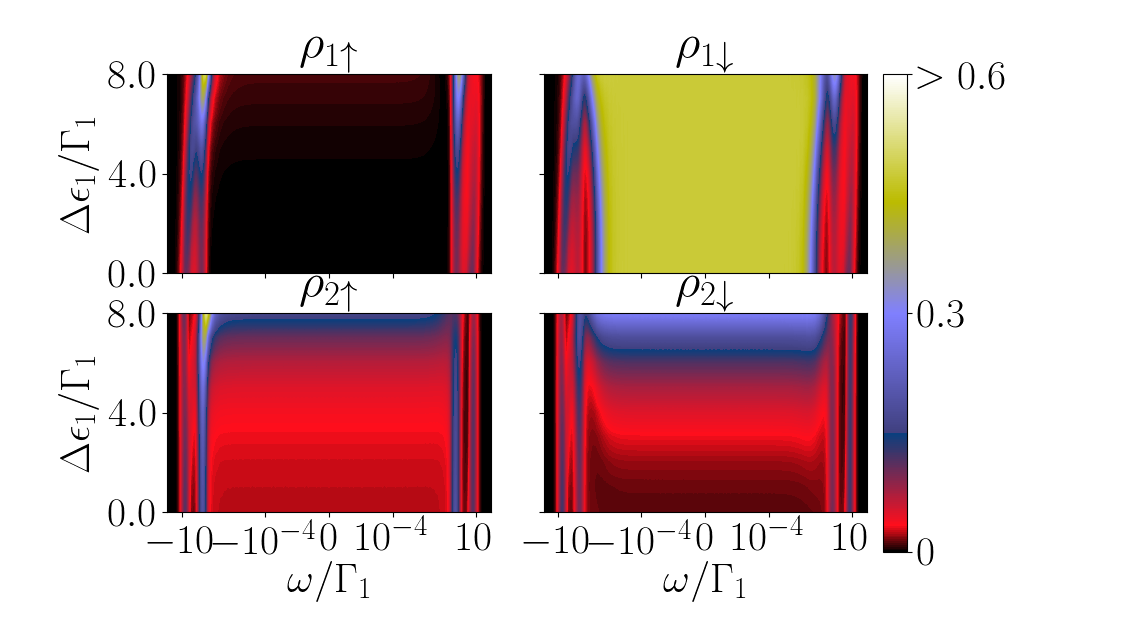
\includegraphics[scale=0.4]{IMAGES/NRG/c)LogEv-ed1.png}
    \caption{\label{fig:logc}  Logarithmic dependence of the density of states for interacting dots coupled in series  \ref{fig:MajoranaModels}(c) over $\omega$ and the gate voltage $\Delta \epsilon_1$. $\Delta \epsilon_2=0$. The dependence over $\Delta \epsilon_2$ produces similar results. \protect\Source{}}
\end{figure}



% -------------------FIGURES EVOLUTION ED--------------------
% \begin{figure}[h]
% \centering
% 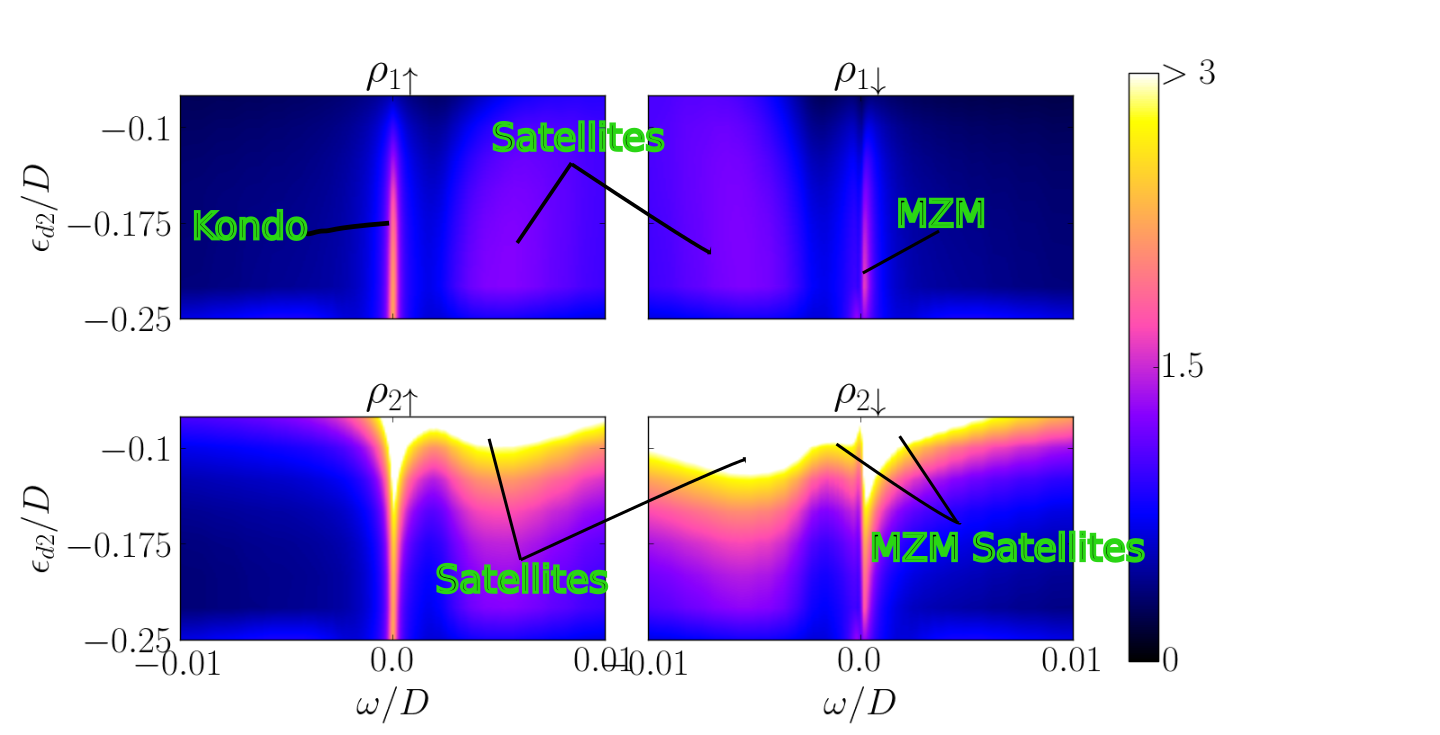
\includegraphics[scale=0.35]{IMAGES/ed2/2D.png}
% \caption{\label{fig:2D/Shift_ed2} Evolution of the DOS of both QDs through the $\ed{2}$ tuning. UP: QD1. DOWN: QD2. LEFT: Spin $\up$. RIGHT: Spin $\dw$.}
% \end{figure}



% -------------------FIGURES EVOLUTION ED--------------------


%-----------E N D  F I G U R E  4 ------
\begin{figure}[bt]
    \begin{center}
    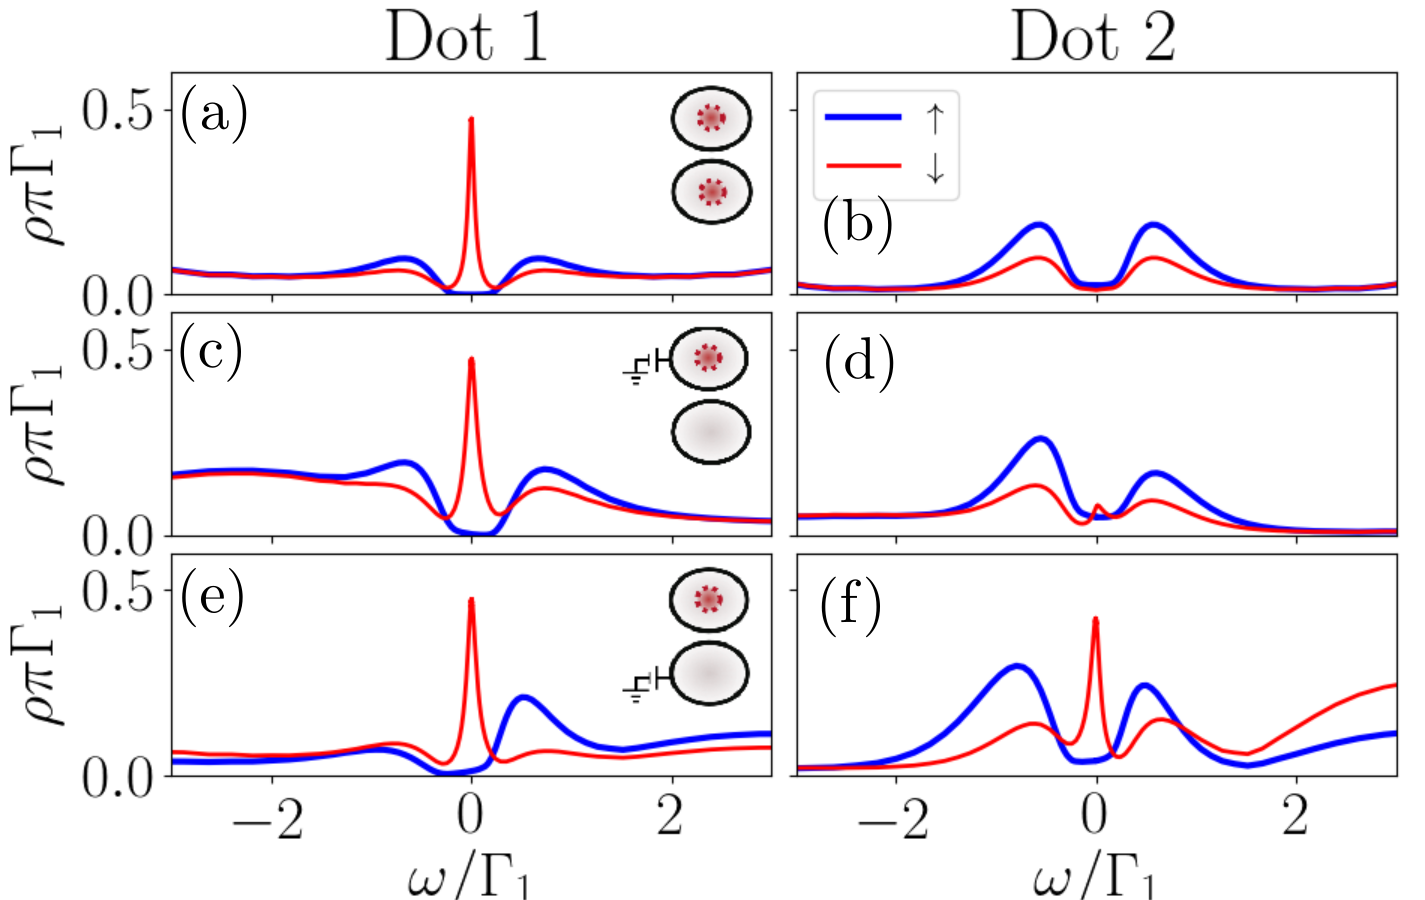
\includegraphics[scale=0.41]{IMAGES/NRG/t2>0.png}
    \caption{  \label{fig:Nt2>0} The same as in \ref{fig:t1=t2} for the  interacting DOS for interacting dots coupled in series (\ref{fig:MajoranaModels}(c)). Inset in b): Zoom to low-energy DOS. \protect\Source{}
    }
    %
    \end{center}
    \end{figure}



    Finally, \ref{fig:Nt2>0} shows the NRG results for the last configuration, where the dots are coupled in series \ref{fig:MajoranaModels}(c). Notably, the indirectly-attached MZM exhibits a robust type II Majorana signature in the first dot over a destroyed Kondo peak. This is observed clearly in  \ref{fig:logc} where $\rho_{1\dw}$ exhibits a constant $\frac{0.5}{\pi \Gamma_1}$-height Majorana peak  . This signature is stable under the gate voltage tuning in dot $1$ and similar results are obtained in dot $2$ . In addition, only  in the particle hole symmetric case the second dot presents a type II Majorana signature (Inset \ref{fig:Nt2>0}(b)). 

    We could understand this effect by thinking that the dots in model (c) are attached in series. Therefore both QDs can be thought as extensions of the Kitaev chain, were the first dot is the last place in the wire. Hence the Majorana should be localized at this dot despite the application of gate voltages. This situation is similar to the case of a single dot attached to a Majorana chain, where it is known that the MZM appears in the dot even when this is supposed to be empty \cite{vernek_subtle_2014}. It still remains the doubt about why this effect is not observed in the non-interacting case . On the other hand, there is a fano resonance at the Fermi energy in the spin-$\dw$ DOS  \ref{fig:Nt2>0}(d)(e) . This zero mode was not identified as a potential Majorana signature since it varies with the values of $\Delta \ep_1$ (\ref{fig:logc}) and $\Delta \ep_2$.
    

We are now writing a paper summarizing these results. As we observed, we were able to characterize the transitions of the Majorana signature in different geometric arrangements of the dots. In the following section we will present some ideas that are still in development. We hope they could lead us to future publications

\section{Additional  results}

\begin{figure}[t]
\centering
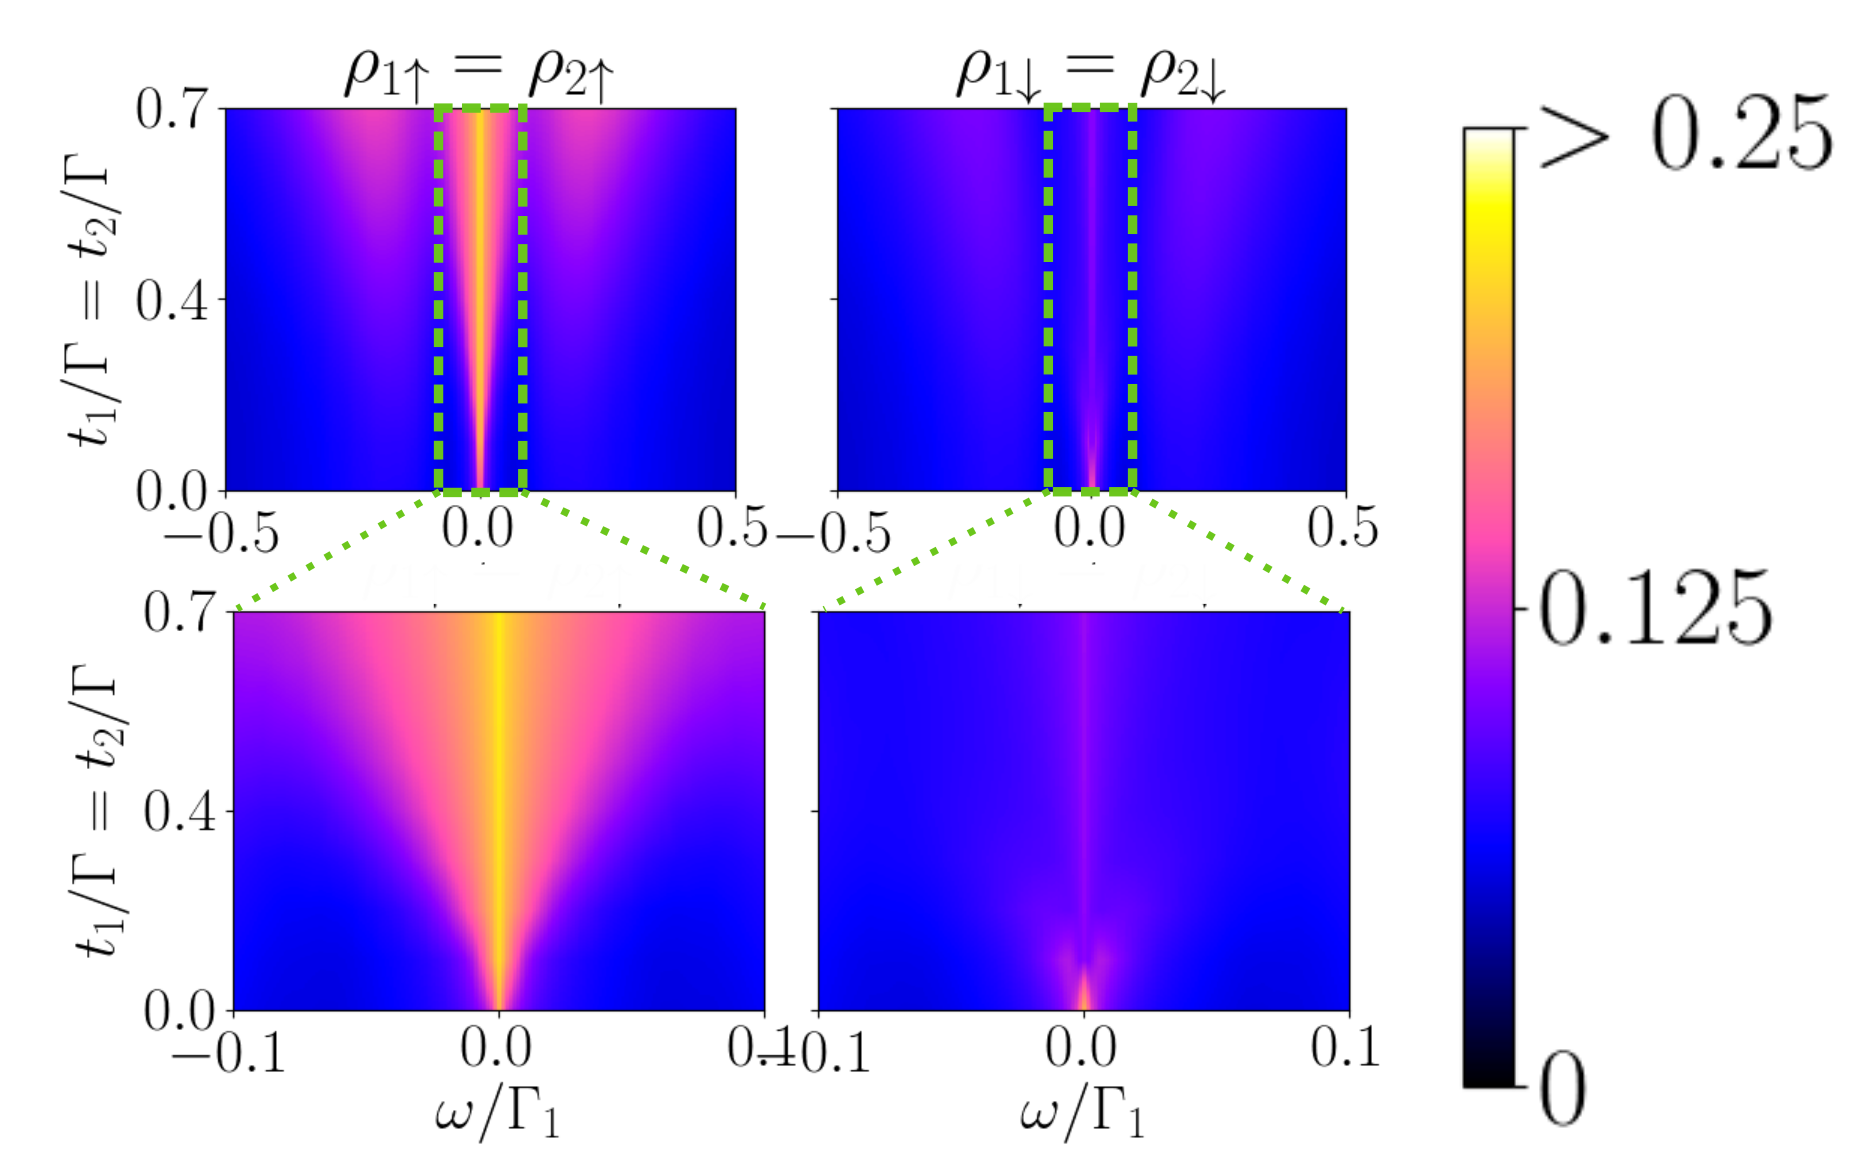
\includegraphics[scale=0.45]{IMAGES/NRG/Indirect.png}
\caption{\label{fig:indirect} Dependence of the DOS in the symmetric model \ref{fig:MajoranaModels}(a) over $t_1=t_2$ and $\omega$. Up: High energy . Down: Zoom to low energy states.  \protect\Source{}}
\end{figure}

This section contains additional results which we are considering to study in  future publications. 

\subsection{Indirect exchange through the Majorana mode}

In \ref{fig:NRG_Majorana} we observed the emergence of satellite peaks at low energies product of anti-ferromagnetic exchange interactions. This exchange interaction can occur through the lead and through the Majorana mode. The reason why we are observing just two satellites is because the Majorana  couplings $(t_1=t_2)$ and the broadening parameters $(\Gamma_1 = \Gamma_2)$ are about the same order. Hence the peaks are a superposition of both exchange interactions. 

We can separate both exchange interactions by observing the dependence of the DOS at different orders of $t_1=t_2$ in \ref{fig:indirect}. We can distinguish two regimes:

\begin{figure}[t]
\centering
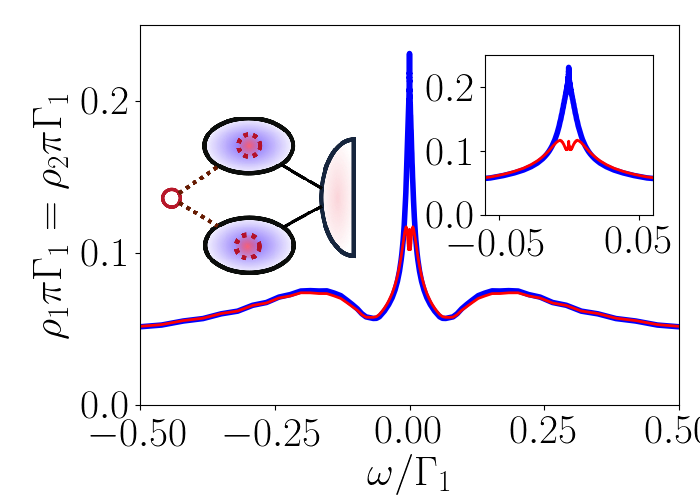
\includegraphics[scale=0.5]{IMAGES/NRG/Lowt1=t2.png}
\caption{ \label{fig:indirectLow} Dependence of the DOS in the symmetric model \ref{fig:MajoranaModels}(a) over $t_1=t_2$ and $\omega$. Up: High energy . Down: Zoom to low energy states.  \protect\Source{}}
\end{figure}

\begin{enumerate}
 \item Low Majorana coupling $t_1=t_2 < 0.5$: Two additional satellite peaks appear in the spin-$\dw$ DOS (See inset in \ref{fig:indirectLow} for better appreciation). These peaks are similar to the  Kondo satellites that appear at high energies. However, since they appear only at low-energies, it is clear that they are produced by the MZM. We conclude that these two satellites are produced by the indirect exchange through the attached  Majorana quasi-particle. 
 \item High Majorana coupling $t_1=t_2 > 0.5$: When the Majorana coupling is high enough, the indirect exchange through the MZM occurs in the same energy scale as the Kondo satellites. Notably, the spin-$\dw$ satellite peaks in the high energy regime are not affected by this effect. Instead, a visible inflation of the satellites in the spin-$\up$ DOS is observed. Therefore the MZM is actually correlated with the spin-$\up$ DOS through the satellite peaks. This is unexpected since the Majorana is only coupled to the spin-$\dw$ channel.  The only explanation for this is that these satellites are formed by a strongly correlated state between the MZM, the dot states and the lead. 
\end{enumerate}
\begin{figure}[h]
\centering
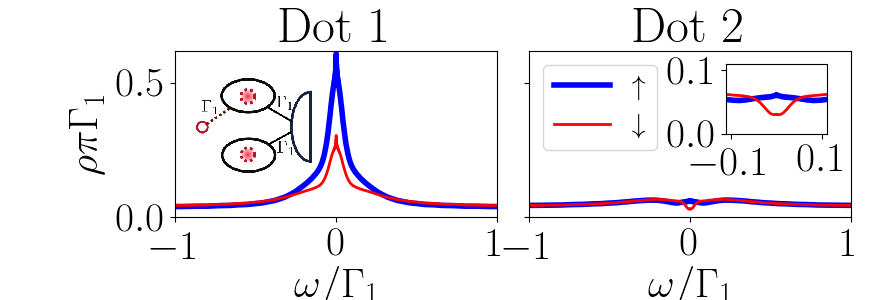
\includegraphics[scale=0.64]{IMAGES/NRG/IND.png}
\caption{\label{fig:IND} DOS at both dots for the model in the left inset. The right inset zooms the low-energy DOS in the second dot.\protect\Source{} }
\end{figure} 

% \begin{figure}[t]
% \centering
% 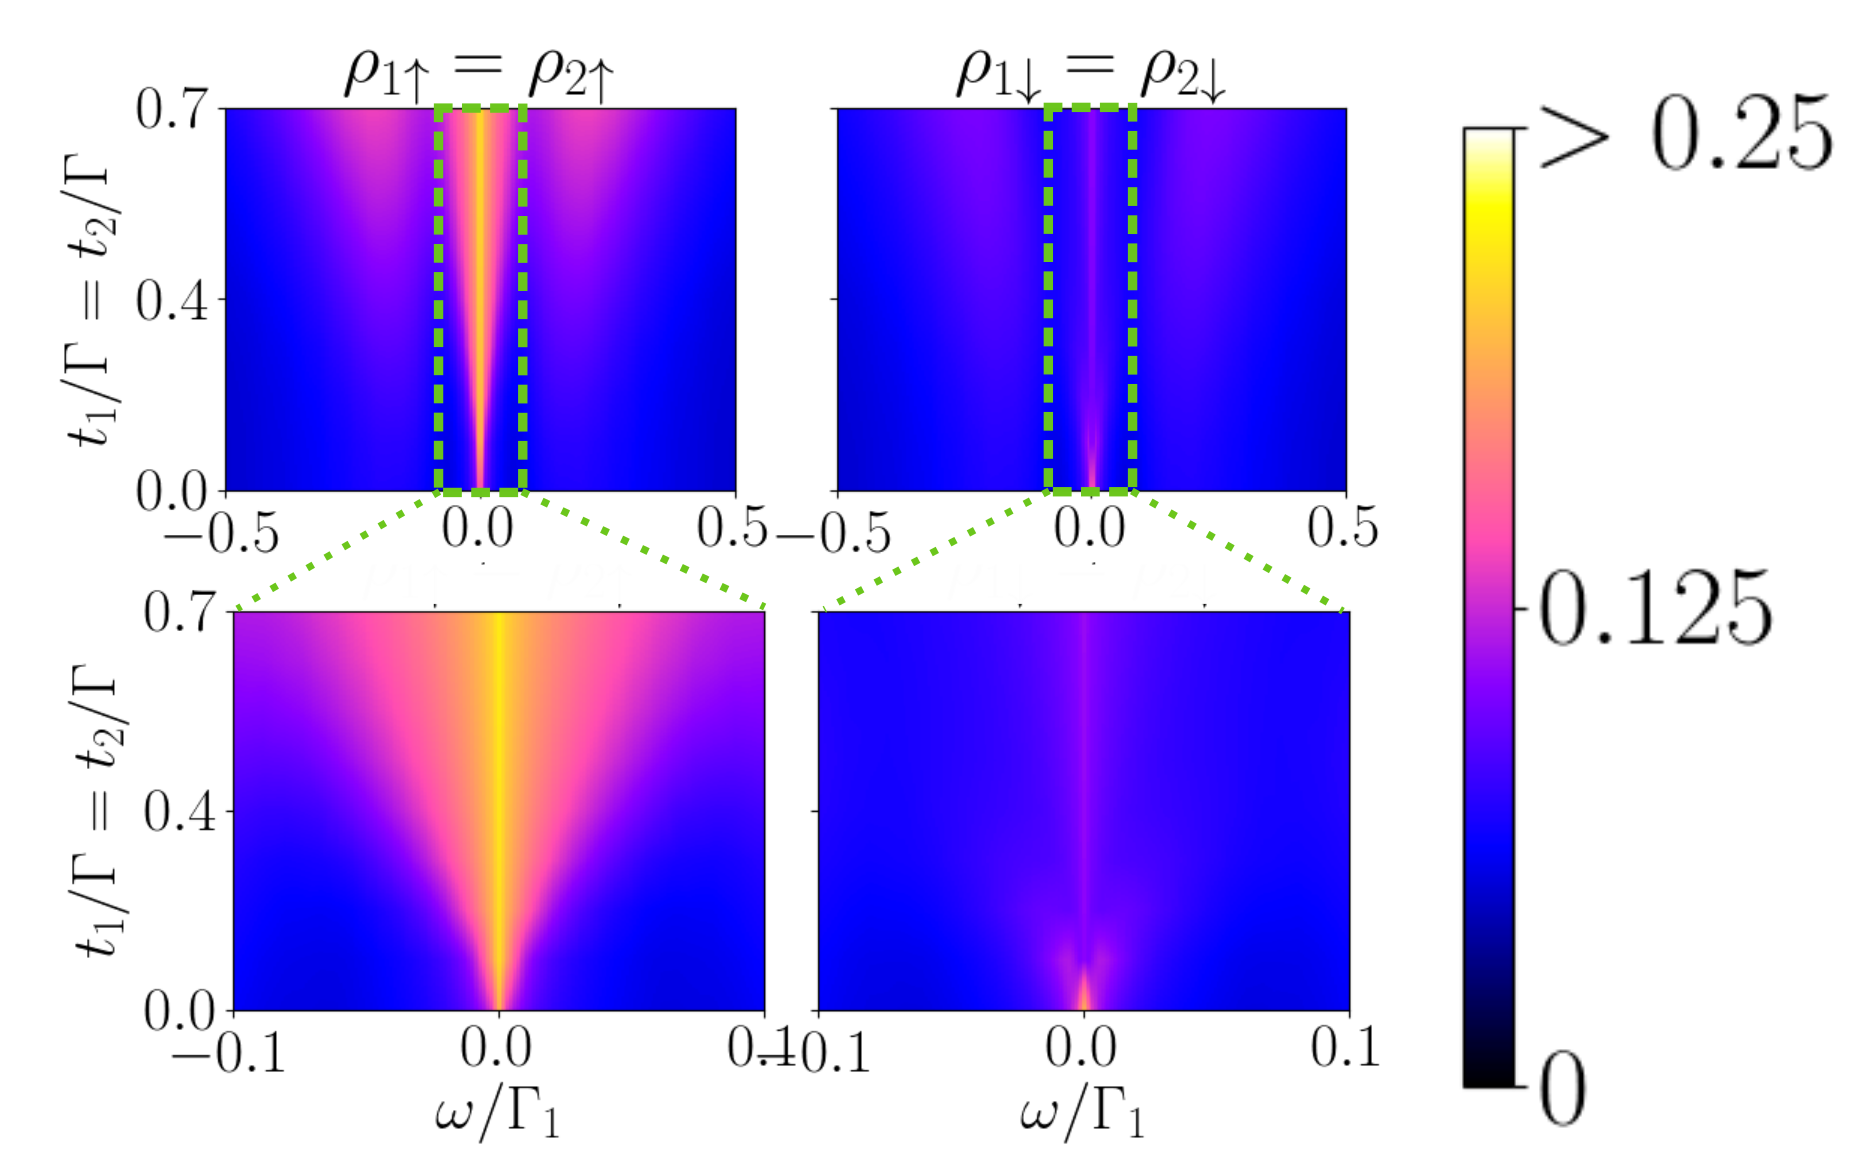
\includegraphics[scale=0.6]{IMAGES/NRG/Indirect.png}
% \caption{\label{fig:indirectLow} Dependence of the DOS in the symmetric model \ref{fig:MajoranaModels}(a) over $\omega$ for $t_1=t_2 = 0.1\Gamma_1$ (Low energy regime). Left inset: Majorana model. Right inset:Low energy regime. Majorana exchange peaks can be observed.  \protect\Source{}}
% \end{figure}



\subsection{Indirect Majorana coupling through the lead}

Imagine a model were we connect both dots symmetrically to the leads but we only connect the MZM to the first dot. In addition, we do not allow inter-dot tunneling. Then the only connection between the MZM and the second dot would be passing through the first dot and  the lead. We didn't expect to see any Majorana signature in the second dot in these conditions. However, \ref{fig:IND} shows a clear type I Majorana signature in the second dot.




 Note also that the density of states in the second dot is very small in comparison with the first dot. This is intriguing since this dot is directly connected with the lead and it is still at the Kondo regime. This ambiguity means that the zero-bias DOS is favored by a direct coupling to an MZM.  

\subsection{Critical behavior in  zero-bias DOS }

In \ref{fig:Nt1>0}(f) we observe a sharp peak at DOS. This peak is actually a big problem for our results since they are  supported on the spectral densities at the Fermi energy. In \ref{fig:Critical} we observe a critical behaviour in the zero-bias DOS close to $\Delta\epsilon_2 =0$. This is quite intriguing . 


\begin{figure}[t]
\centering
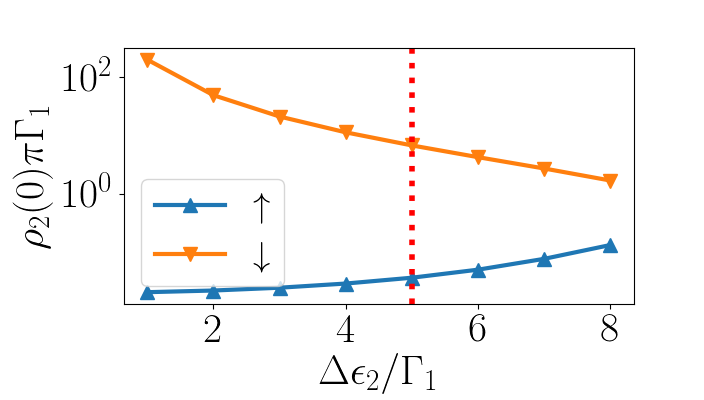
\includegraphics[scale=0.6]{IMAGES/NRG/Critical.png}
\caption{\label{fig:Critical} Logarithmic dependence of the DOS in the second dot for setup in \ref{fig:MajoranaModels}(b) over the second gate voltage. Cut at $5\Gamma_1$ corresponds to \ref{fig:Nt1>0}(f). \protect\Source{} }
\end{figure} 
%$U_{1}=U_{2}=-2\epsilon_{d1}=-2\epsilon_{d2}=0.5$, %$\Gamma_{1}=\Gamma_{2}$,
%$t_{1}=0.02$

% \begin{figure*}[h]
% \centering
% 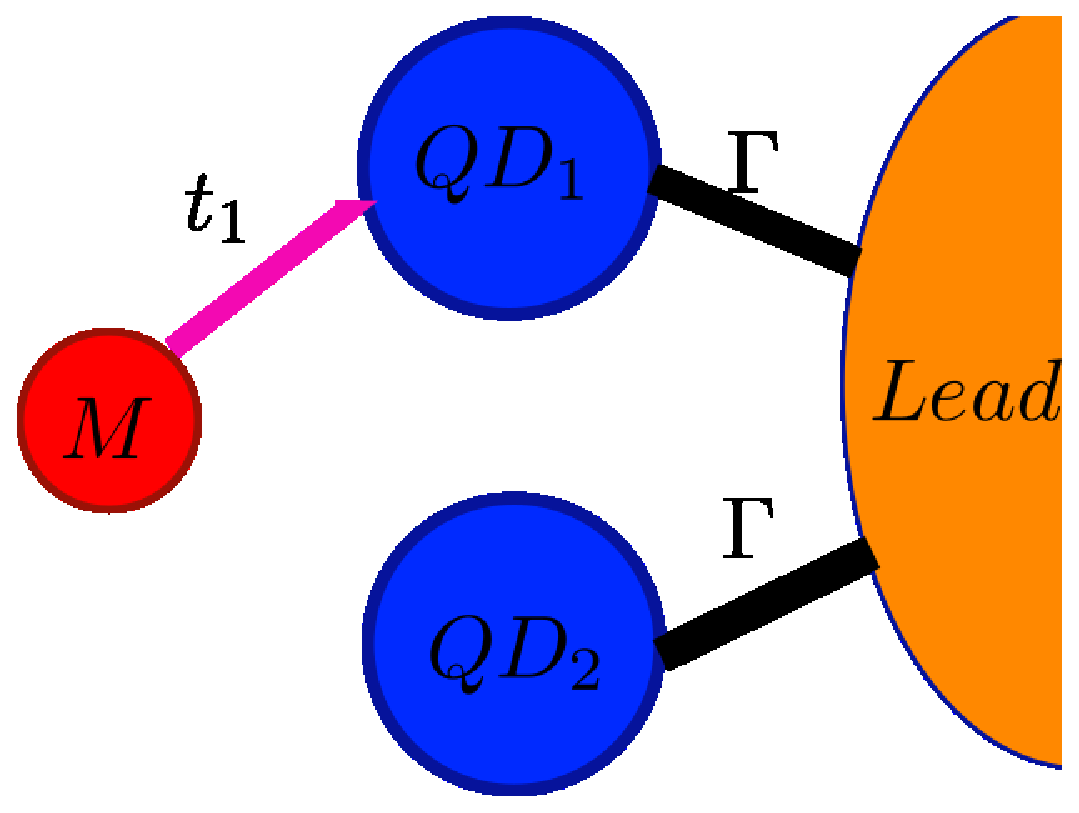
\includegraphics[scale=0.2]{Plots/Model/Majorana-1QD.eps}
% \caption{\label{fig:Mod/Shift_t2}$U_{1}=U_{2}=-2\ep_{d1}=-2\epsilon_{d2}=0.5$, $\Gamma_{1}=\Gamma_{2}$,
% $t_{1}=0.02$. Variable $t_2$}
% \end{figure*}


% \begin{figure}[hbt]
% \centering
% 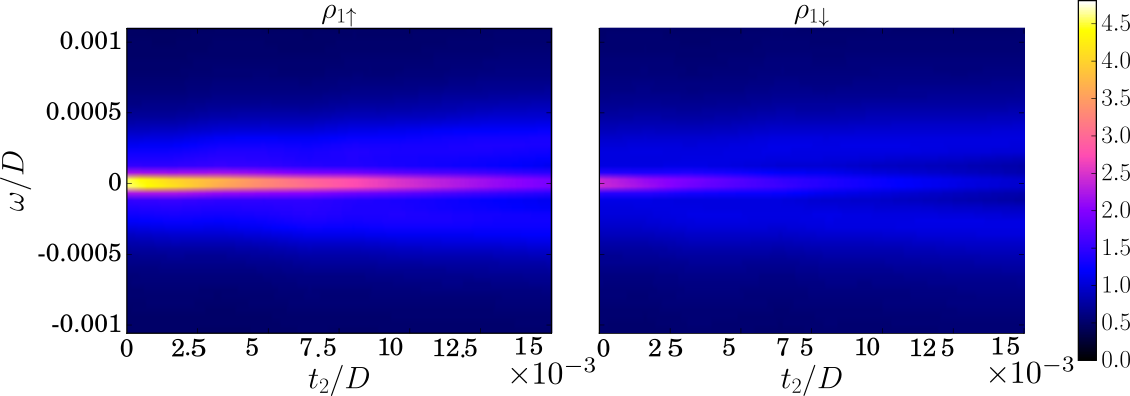
\includegraphics[scale=0.38]{Plots/2D/Shift_t2D1.png}
% \caption{\label{fig:DOS/Shift_t2D1} Evolution of the DOS in the first QD }
% \end{figure}
% % \begin{figure}[hbt]
% % \centering
% % 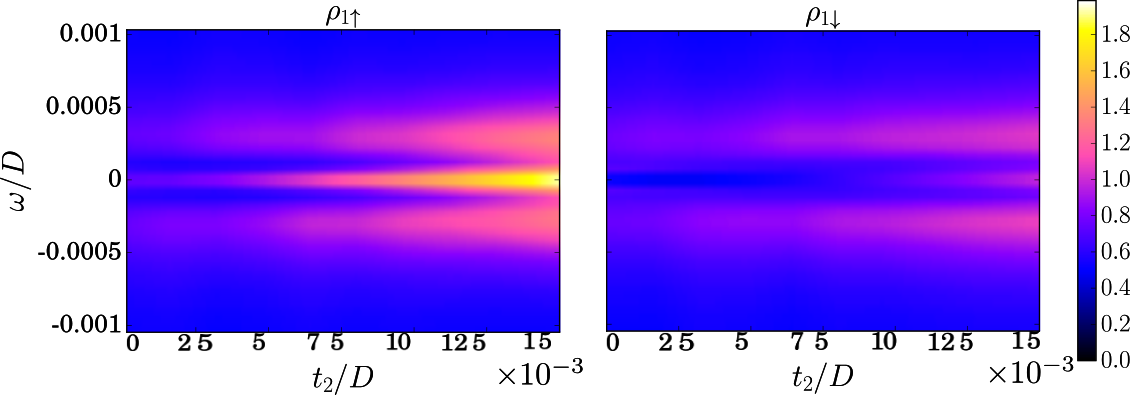
\includegraphics[scale=0.38]{Plots/2D/Shift_t2D2.png}
% % \caption{\label{fig:DOS/Shift_t2D2} Evolution of the DOS in the Second QD}
% % \end{figure}



% \iffalse
% \begin{figure}[hbt]
% \centering
% 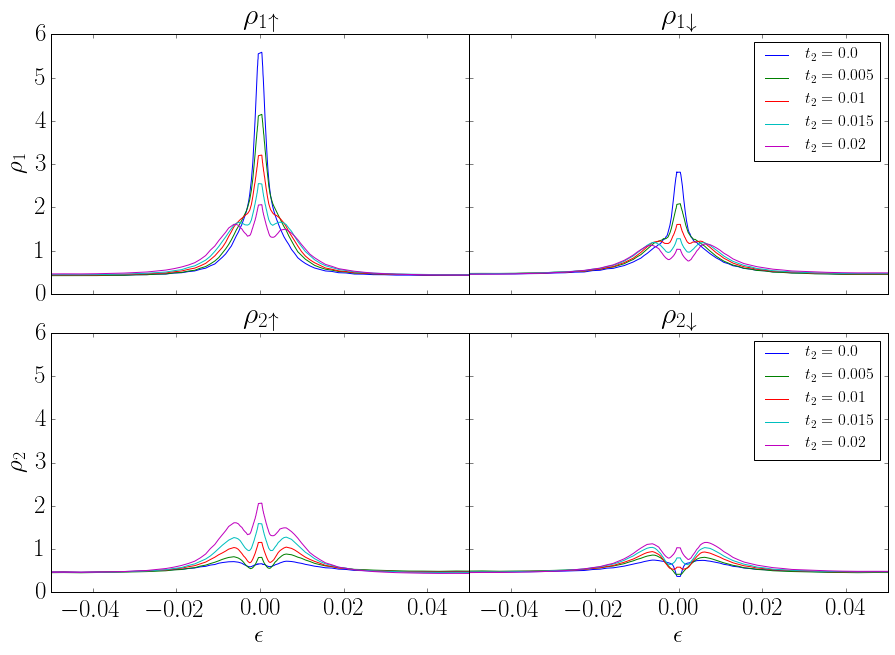
\includegraphics[scale=0.38]{Plots/DOS/Shift_t2.png}
% \caption{\label{fig:DOS/Shift_t2} Evolution of the QDs' DOS for the procedure in \ref{fig:Mod/Shift_t2} }
% \end{figure}
% \fi
%  In \ref{fig:DOS/Shift_t2D1} and \ref{fig:DOS/Shift_t2D1} we observe the evolution of DOS in the case where the second dot is smoothly connected to the Majorana, which is already attached to the first dot. The hopping parameter $t_2$ scales up to $0.015D$ where the model reaches the symmetry $t_2 = t_1$. The figures show that increasing $t_2$ leads to a drop in the DOS of QD1 while the DOS in QD2 is increased. In addition, the single peak in the first dot transforms into a three-peak due to the Majorana interference with the second dot. In \ref{fig:MSig/Shift_t2} we also observe that the reason between the zero up-down DOS  $\left(\frac{\rho_\up(0)}{\rho_\up(0)}\right)$ smoothly scales up to $2$ in QD2. At $t_2 =0.02$, when the  is completely symmetric, the Majorana signature appears in both quantum dots. Note that the relation $\frac{\rho_\up(0)}{\rho_\up(0)}$  is already close to $2$ at $t_2=0$. This implies that the second dot "feels" the Majorana even when it is not directly connected to the Majorana mode. 















% %-----------E N D  F I G U R E  4 ------


% %-----------F I G U R E  t1 =t2 ------

% \begin{figure}[hbt]
% \centering
% 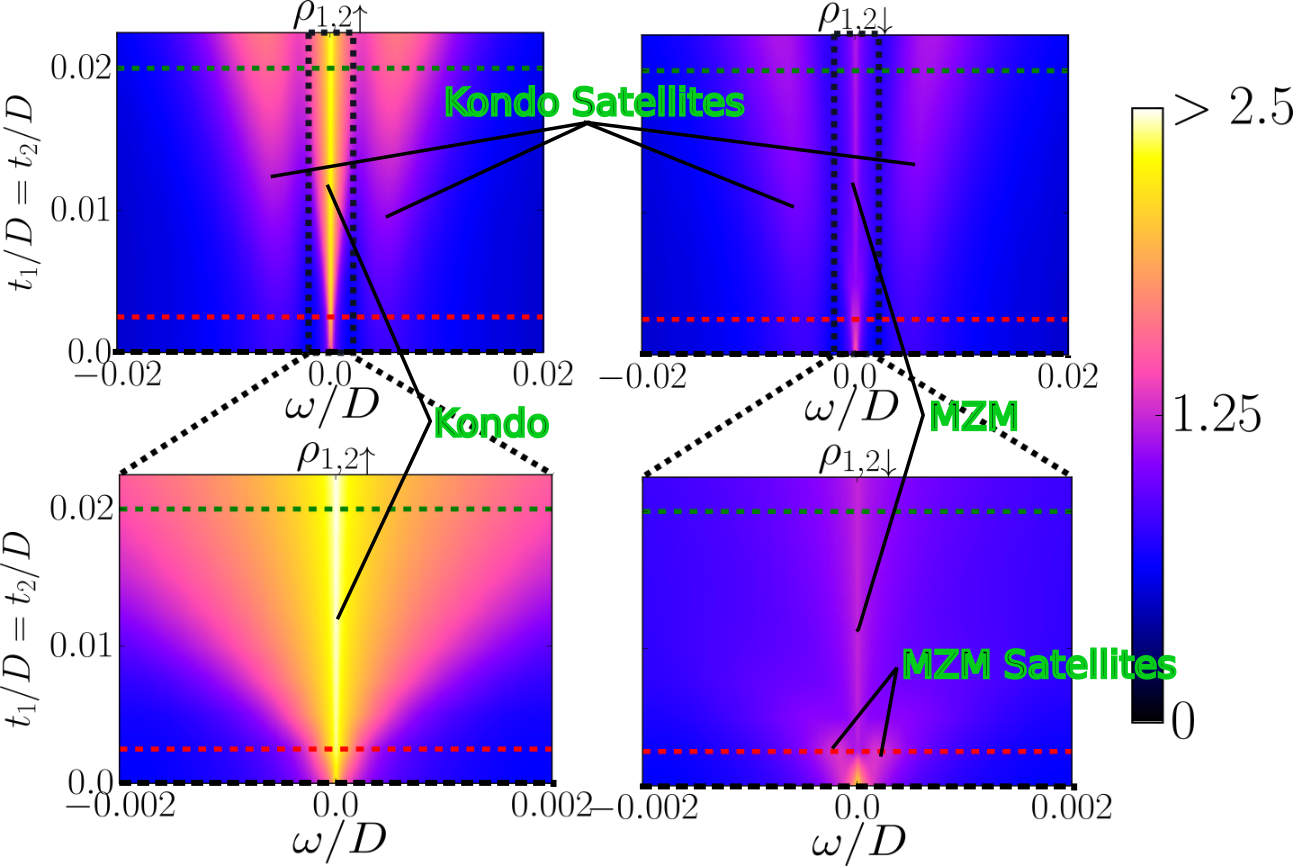
\includegraphics[scale=0.35]{IMAGES/t1=t2/2D.png}
% \caption{\label{fig:2D/Shift_t1=t2} Evolution of the DOS of both QDs through $t_1 = t_2$ tuning. UP: Energy scale $\omega \sim 10^{-2}D$. DOWN: Energy scale $\omega \sim 10^{-3}D$. LEFT: Spin $\up$. RIGHT: Spin $\dw$.}
% \end{figure}



%  %-----------F I G U R E  t1=t2 ------
% \begin{figure}[bt]
%     \begin{center}
%     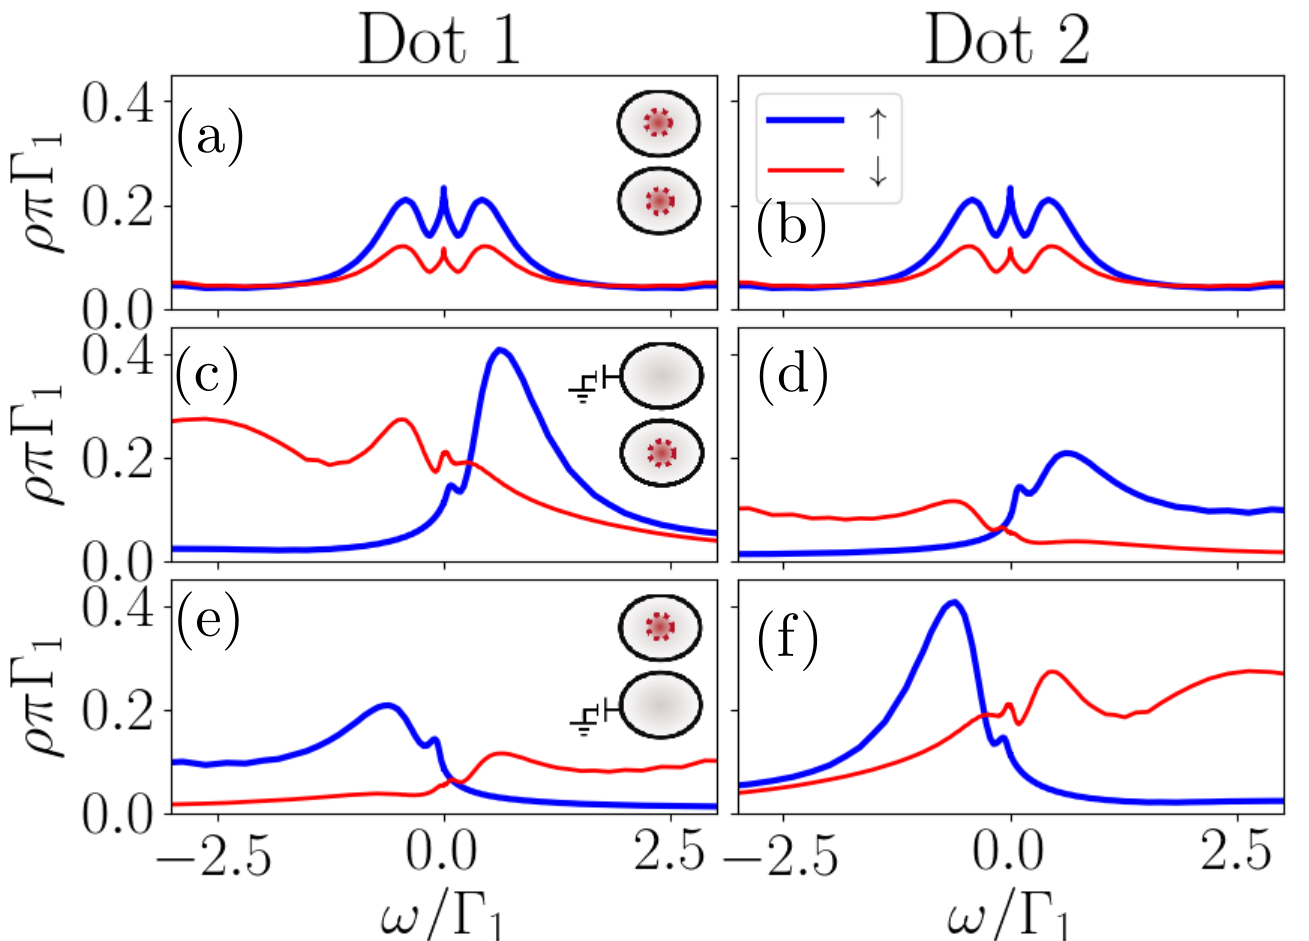
\includegraphics[scale=0.45]{IMAGES/NRG/t1=t2.png}
%     \caption{  \label{fig:NRG_SymCoupling} Density of states in dots 1(Left) and 2(Right) for the model \ref{fig:Models}. (a). First line (a),(b): $\ep_1=\ep_2=0$. Second line (c),(d): $\ep_1=5\Gamma_1$ , $\ep_2=0$. Third line (e),(f): $\ep_2=-5\Gamma_1$ , $\ep_1=0$.   Blue bold lines: Spin-$\up$ DOS. Red thin lines: Spin-$\dw$ DOS. The inset at the upper-right corner of each line indicates which dots  exhibit  Majorana signature, which is represented by a red dashed circle inside the dot. 
%     }
%     %
%     \label{fig:t2>0}
%     \end{center}
% \end{figure}
% %-----------F I G U R E  t1 =t2 ------


%  %-----------F I G U R E  t1 >0 ------
% \begin{figure}[bt]
%     \begin{center}
%     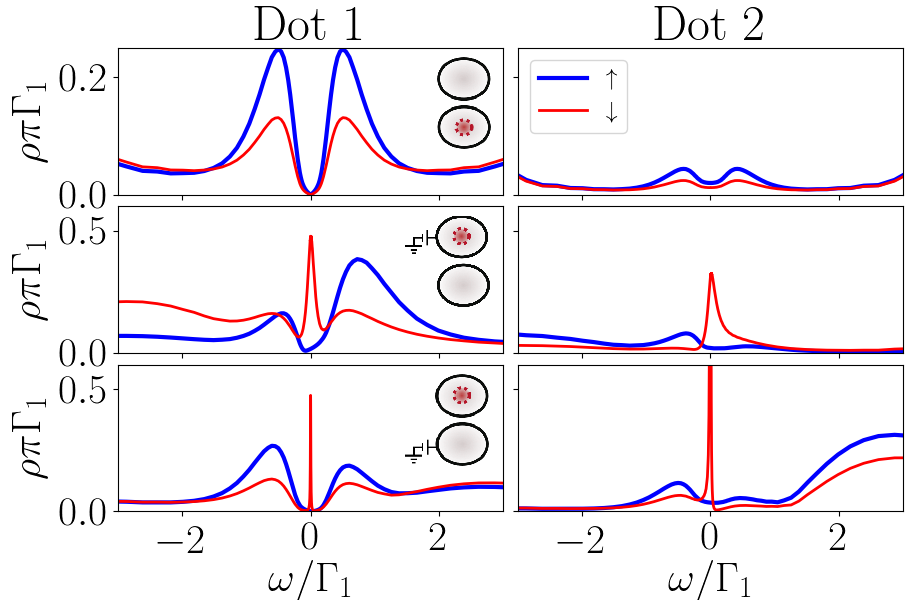
\includegraphics[scale=0.45]{IMAGES/NRG/t1>0.png}
%     \caption{   \label{fig:NRG_Interference} Density of states in dots 1(Left) and 2(Right) for the model \ref{fig:Models}. (b). First line (a),(b): $\ep_1=\ep_2=0$. Second line (c),(d): $\ep_1=5\Gamma_1$ , $\ep_2=0$. Third line (e),(f): $\ep_2=-5\Gamma_1$ , $\ep_1=0$.   Blue bold lines: Spin-$\up$ DOS. Red thin lines: Spin-$\dw$ DOS. The inset at the upper-right corner of each line indicates which dots  exhibit  Majorana signature, which is represented by a red dashed circle inside the dot. 
%     }
%     %
%     \label{fig:t2>0}
%     \end{center}
% \end{figure}
% %-----------F I G U R E  t1 >0 ------



%  %-----------F I G U R E  t2 >0 ------
% \begin{figure}[bt]
%     \begin{center}
%     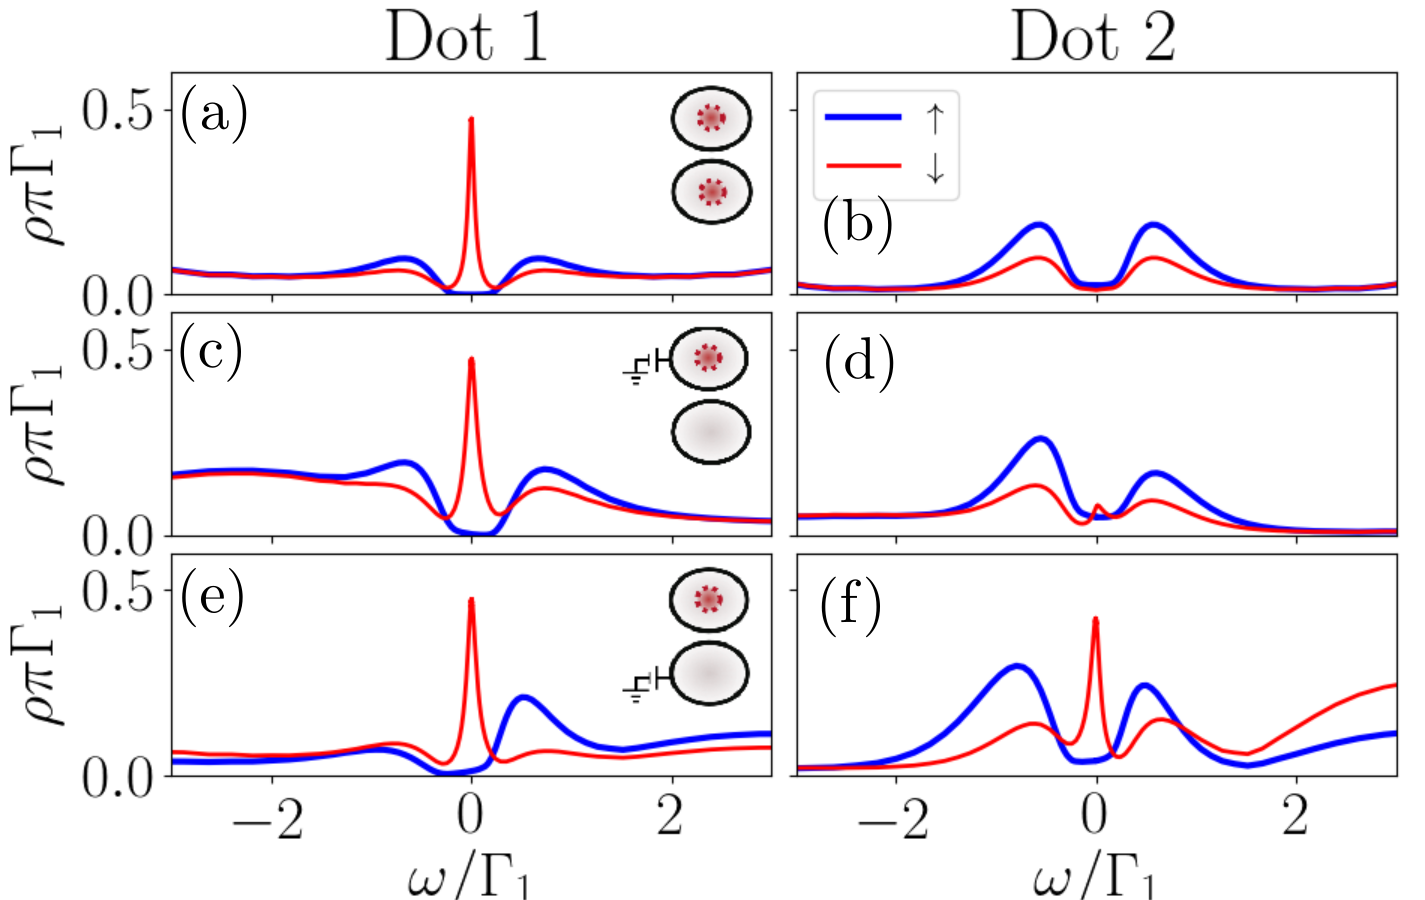
\includegraphics[scale=0.45]{IMAGES/NRG/t2>0.png}
%     \caption{  \label{fig:NRG_IndirectCoupling} Density of states in dots 1(Left) and 2(Right) for the model \ref{fig:Models}. (c). First line (a),(b): $\ep_1=\ep_2=0$. Second line (c),(d): $\ep_1=5\Gamma_1$ , $\ep_2=0$. Third line (e),(f): $\ep_2=-5\Gamma_1$ , $\ep_1=0$.   Blue bold lines: Spin-$\up$ DOS. Red thin lines: Spin-$\dw$ DOS. The inset at the upper-right corner of each line indicates which dots  exhibit  Majorana signature, represented by a red dashed circle inside the dot. 
%     }
%     %
%     \label{fig:t2>0}
%     \end{center}
% \end{figure}
% %-----------F I G U R E  t2 >0 ------


% {}

%  %-----------F I G U R E  4 ------
% \begin{figure}[bt]
% \begin{center}
% \includegraphics[scale=0.48]{Graficos/t2=0.png}
% \caption{  \label{fig:Interference} Density of states in both dots of the case where the only the first QD is attached to both Majorana and Lead (\ref{fig:MajoranaModels} second column) . Solid lines: Spin-$\up$ DOS. Dashed lines: Spin-$\dw$ DOS.
% }
% %
% \label{fig:GenModel}
% \end{center}
% \end{figure}
% %-----------E N D  F I G U R E  4 ------

%  %-----------F I G U R E  4 ------
% \begin{figure}[bt]
% \begin{center}
% \includegraphics[scale=0.48]{Graficos/t2=0.png}
% \caption{  \label{fig:Interference} Density of states in both dots of the case where the only the first QD is attached to both Majorana and Lead (\ref{fig:MajoranaModels} second column) . Solid lines: Spin-$\up$ DOS. Dashed lines: Spin-$\dw$ DOS.
% }
% %
% \label{fig:GenModel}
% \end{center}
% \end{figure}
% %-----------E N D  F I G U R E  4 ------




% \newpage


% % -------------------------------------------------------------
% \subsection{ a) Removing Kondo and Majorana with QD-interference \label{sec:a)}}
% \Jesus{Text coming soon}

% \begin{figure}[H]
%     \centering
%     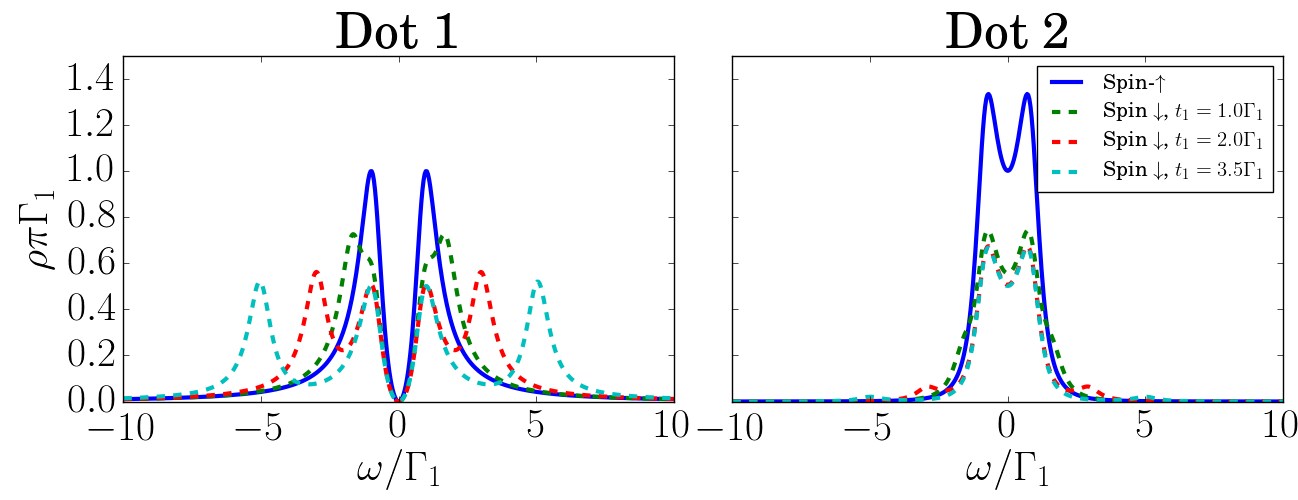
\includegraphics[scale=0.35]{IMAGES/DQD-M/a)}
%     \caption{\label{fig:a)} \protect\Source{   }}
% \end{figure}

%  \begin{figure}[H]
%      \centering
%      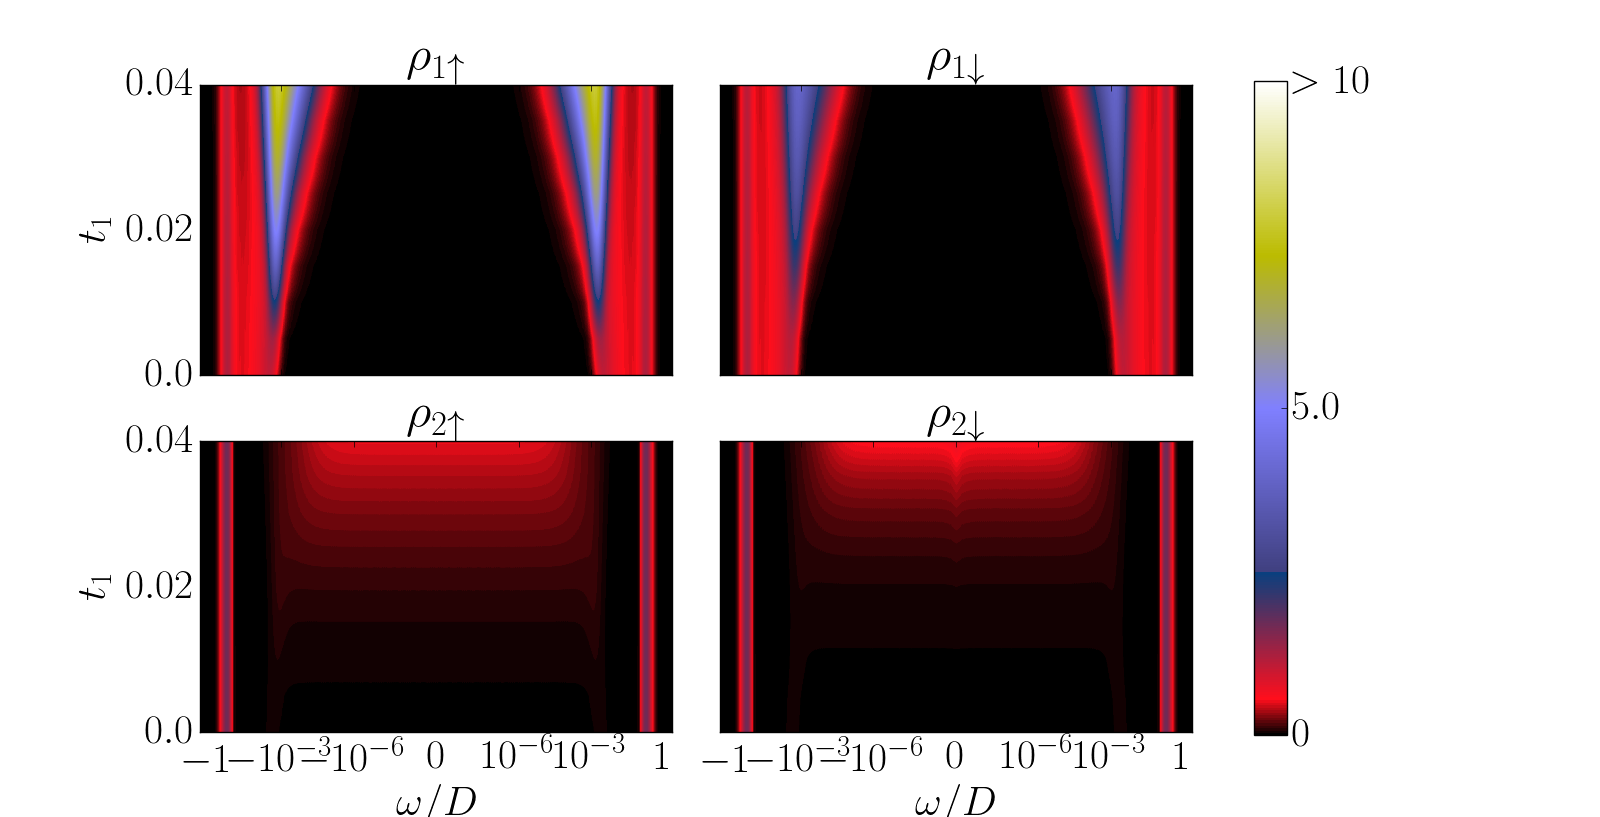
\includegraphics[scale=0.35]{IMAGES/DQD-M/a)-NRG.png}
%      \caption{\label{fig:a)NRG} \protect\Source{   } }
% \end{figure}


% % -------------------------------------------------------------
% \subsection{ b) Indirect Majorana after Removing Kondo with QD-interference \label{sec:b)}}
% \begin{figure}[H]
% \centering
% 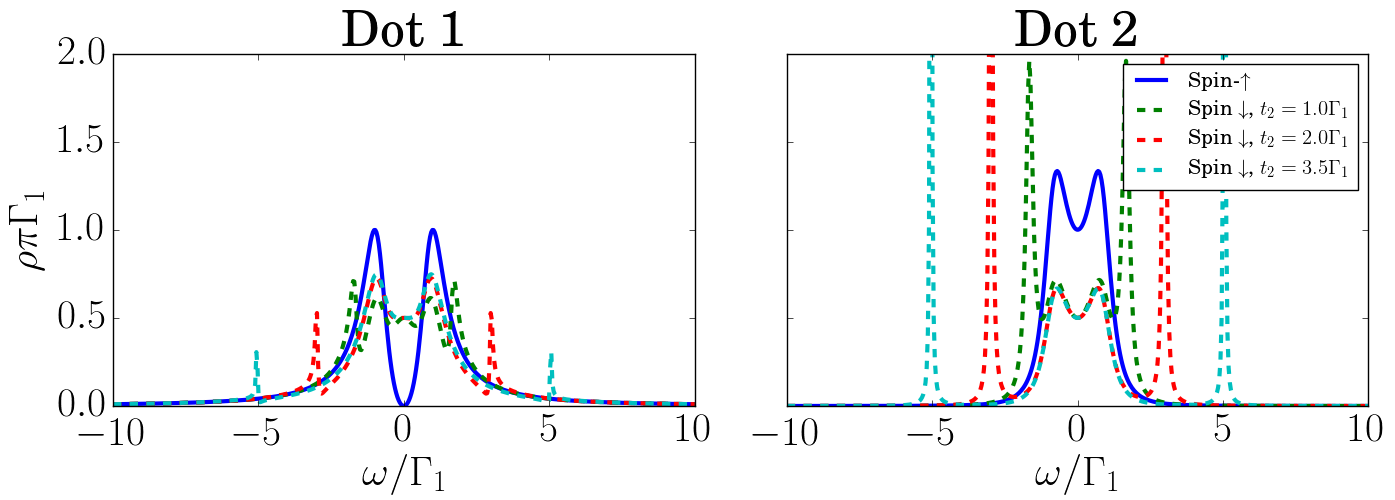
\includegraphics[scale=0.35]{IMAGES/DQD-M/b).png}
% \caption{\label{fig:b)}\protect\Source{   } }
% \end{figure}

% \begin{figure}[H]
%     \centering
%     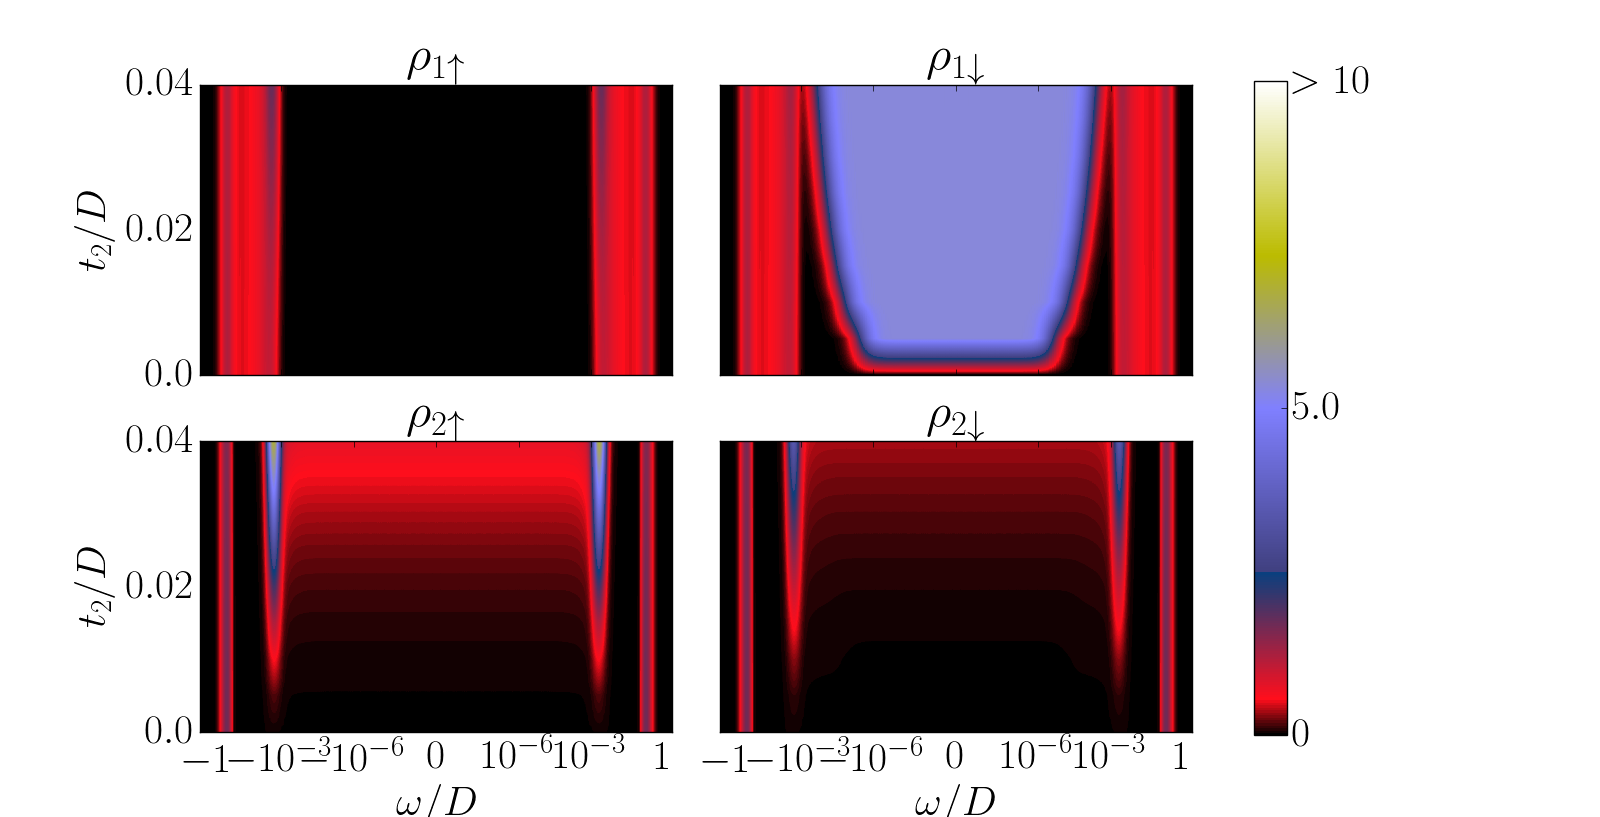
\includegraphics[scale=0.35]{IMAGES/DQD-M/b)-NRG.png}
%     \caption{\label{fig:b)NRG} \protect\Source{   }}
% \end{figure}





% \newpage


% % -------------------------------------------------------------------
% \subsection*{c) Attaching the Majorana mode to the DQD (Tuning $t_1=t_2$) \label{sec:t1=t2}}

% \textbf{Parameters:}

% $$\Gamma \sim 2.83*10^{-2}D, t_{dots}=0 , U_{1,2} = -2\ed{1,2} = 0.5$$
% $$t_1=t_2 \in [0\  ,\  2.5*10^{-2}D]$$

% \begin{figure}[hbt]
% \centering
% 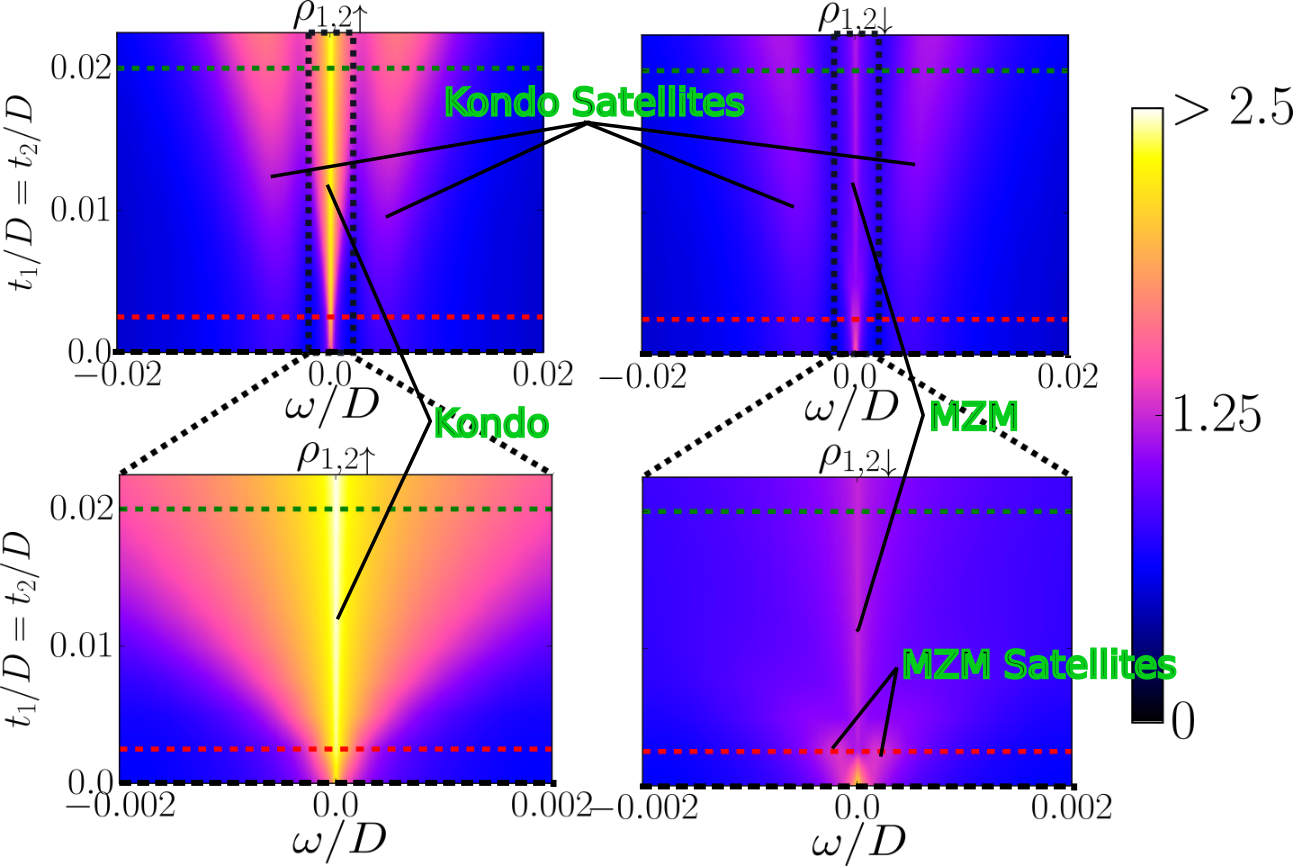
\includegraphics[scale=0.35]{IMAGES/t1=t2/2D.png}
% \caption{\label{fig:2D/Shift_t1=t2} Evolution of the DOS of both QDs through $t_1 = t_2$ tuning. UP: Energy scale $\omega \sim 10^{-2}D$. DOWN: Energy scale $\omega \sim 10^{-3}D$. LEFT: Spin $\up$. RIGHT: Spin $\dw$.}
% \end{figure}



% Consider that we are attaching the MZM to both Quantum Dots symmetrically \ref{fig:MajoranaModels}.(a). For this, we scale up the coupling parameter $t_1=t_2$ from $0$ (Decoupled) to $3\Gamma$ (Completely coupled).The other parameters where chosen with an equilibrium between the dot energy and Coulomb repulsion $(\ed{1,2}=-\frac{U_{1,2}}{2})$  and  without inter-dot coupling $t_{dots}=0$. These circumstances guarantee that the system preserves Particle Hole Symmetry (PHS). Thus the Density of States (DOS) of particles and holes remains equal at all instances $(\rho(-\omega) = \rho(\omega))$. \\

% \begin{figure}[hbt]
% \centering
% 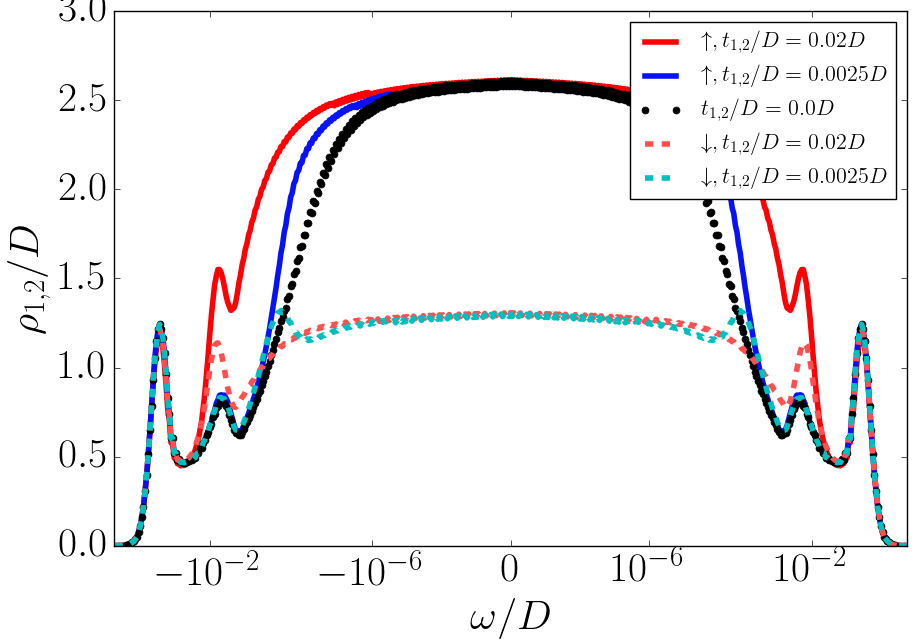
\includegraphics[scale=0.35]{IMAGES/t1=t2/LogPlot.png}
% \caption{\label{fig:t1=t2/logplot} Density of states at each QD of the horizontal dashed cuts in \ref{fig:2D/Shift_t1=t2}. The energy is in logarithmic scale.  For $t_1=t_2>0$ spin-$\up$ and spin-$\dw$ DOS split near the order of $\vert \omega \vert \sim t_1,2 $. At the Fermi energy $(\omega =0)$  $\rho_\up = 2\rho_\dw$ due to the presence of the MZM in both QDs. }
% \end{figure}

% In the case where the Majorana is detached from the DQD $(t_1 =t_2 = 0)$, the system favors the appearance of a three-peak at low energies as it is shown in \ref{fig:t1=t2/logplot} . The central peak is produced only by the Kondo effect and the two other satellite peaks are the result of a strong correlation between both dots caused by the indirect exchange of quantum states through the Lead \ref{sec:DoublePeak}. \\

% Once the MZM the spin-$\up$ and spin-$\dw$ DOS split at low energies due to the new spin-$\dw$ transport channel through the Majorana mode. The spin-$\dw$ DOS at the Fermi energy ($\omega =0$) decays to the half of the spin-$\up$ DOS $\rho_\dw = \frac{\rho_\up}{2} $. By symmetry in the dot parameters this event occurs equally for both QDs. We adopt this fact as a Majorana signature. Hence we obtain that the MZM leaks inside both quantum dots. 

% There is also an additional effect caused by the indirect exchange between the QDs through the Majorana mode . The consequences of this effect depend on the energy range of the Majorana couplings $t_1=t_2$.  : 
% \begin{enumerate}
%     \item If $t_1=t_2 \ll \Gamma $ two more satellites are formed at very low energies ($\sim t_1$) in the spin-$\dw$ DOS (See  \ref{fig:2D/Shift_t1=t2} Spin-down $\omega \sim 10^{-3}D$ ). (See  \ref{fig:2D/Shift_t1=t2} Spin $\up$, $\omega \sim 10^{-3}D$ ).
%     \item If $t_1=t_2 \sim \Gamma$ , the MZM contributes to the the growth of the spin-up satellites in the DOS. This effect produces the splitting between the spin-up and spin-down DOS.   (See  \ref{fig:2D/Shift_t1=t2} Spin-$\dw$, $\omega \sim 10^{-2}D$).
% \end{enumerate}









% % At low energies $(\omega/D \sim 10^{-2})$ \ref{fig:2D/Shift_t1=t2} shows the emergence of a 3-peak in the DOS close to the Fermi energy. This 3-peak is formed by a central peak defined by the Kondo (spin $\up$) and the Majorana (spin $\dw$) peaks. The other two peaks are generated by an indirect exchange of the states between the quantum dots through the leads (SEE ABSTRACT). At even lower energies $(\omega/D \sim 10^{-4})$ it is possible to appreciate the emergence of another 3-peak in the spin down DOS which is present only for small values of the Majorana coupling constants $t_1 = t_2 \ll 0.01D$ (See  \ref{fig:t1=t2/logplot}). These sided peaks are caused by the indirect exchange between both dots through the Majorana Mode. When the Majorana couplings achieve the same order of the dot-lead coupling $\Gamma$ $(t_1 = t_2 \sim  0.01D)$ both sided peaks are merged causing the extinction of the majorana side-peaks and the increase of the indirect exchange peaks at $(\omega/D \sim 10^{-2})$. 

% % \begin{figure}[H]
% % \centering
% % 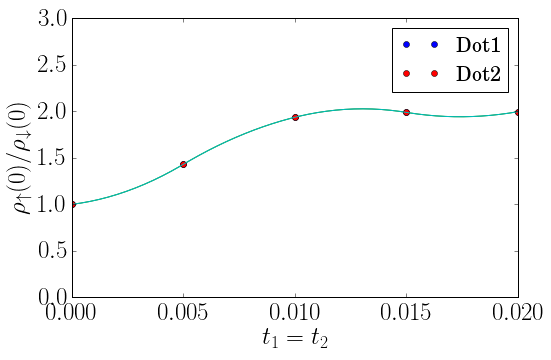
\includegraphics[scale=0.4]{Plots/MSig/Shift_t1=t2.png}
% % \caption{\label{fig:MSig/Shift_t1=t2} Relation between the Zero-peaks at the fermi level. The Majorana signature is related to $\frac{\rho_\up(0)}{\rho_\up(0)}=2$.}
% % \end{figure}










% %--------------------------------------------------------------------

% \subsection{ e) Transferring the MZM through gate voltage shifting $\ed{2}$. \label{sec:e2}}

% \textbf{Parameters:}

% $$\Gamma \sim 2.83*10^{-2}D, t_{dots}=0 , U_{1,2} = -2\ed{1} = 0.5 , t_1=t_2=0.0025$$
% $$\ed{2} \in [-0.25 \  , -0.05]$$

% This process starts with the DQD coupled symmetrically  to the Majorana mode, just as in \ref{sec:t1=t2}. The idea of this process is to break PHS by increasing the energy of the second QD $\ed{2}$. This procedure should induce the Majorana to tunnel only into the first dot. 

% % -------------------FIGURES EVOLUTION ED--------------------
% \begin{figure}[h]
% \centering
% 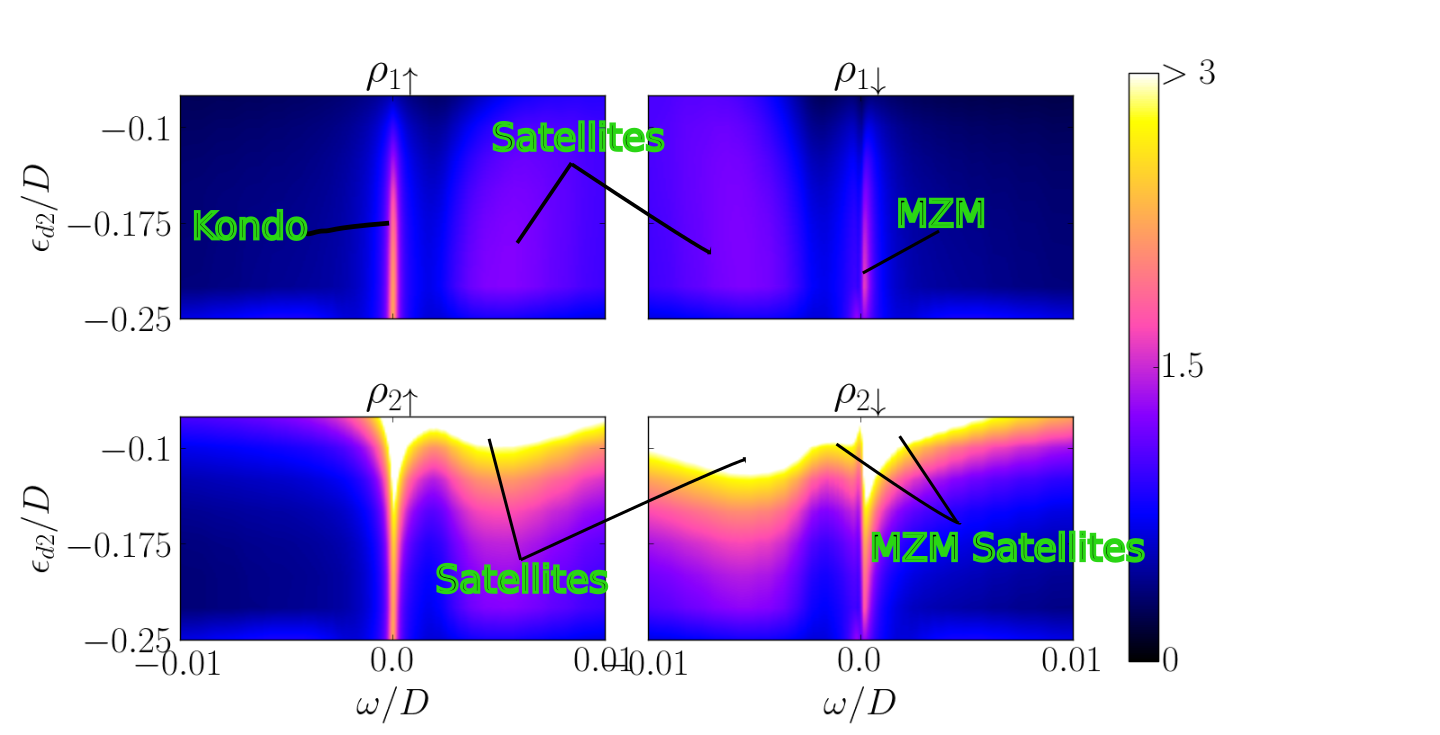
\includegraphics[scale=0.35]{IMAGES/ed2/2D.png}
% \caption{\label{fig:2D/Shift_ed2} Evolution of the DOS of both QDs through the $\ed{2}$ tuning. UP: QD1. DOWN: QD2. LEFT: Spin $\up$. RIGHT: Spin $\dw$.}
% \end{figure}


% \begin{figure}[H]
% \centering
% 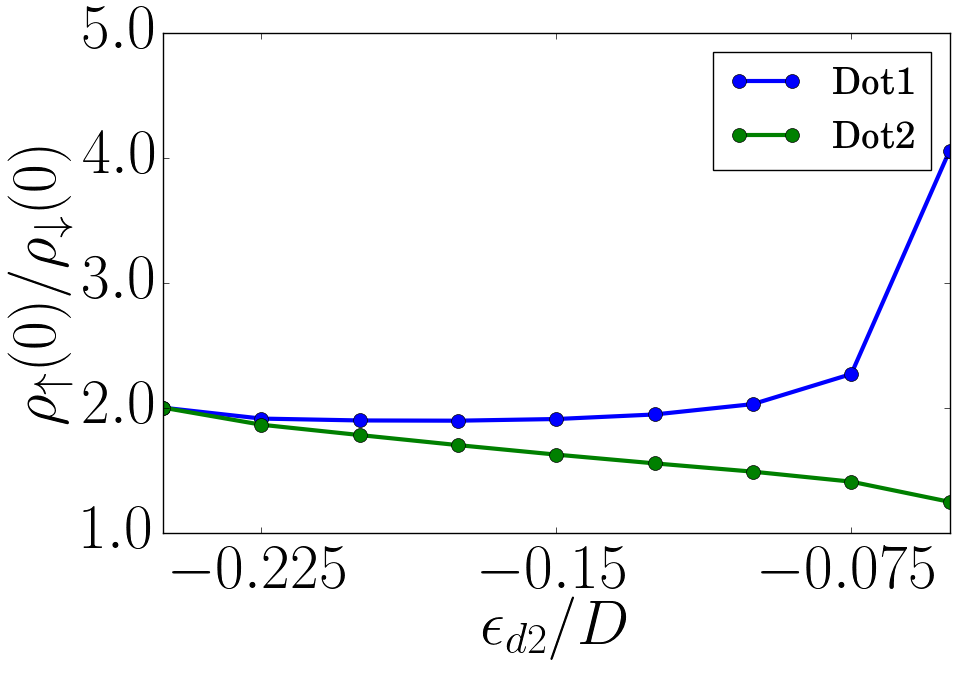
\includegraphics[scale=0.3]{IMAGES/ed2/Fermi.png}
% \caption{\label{fig:ed2/Fermi} As described in \ref{sec:t1=t2} the relation $\frac{\rho_\up(0)}{\rho_\up(0)}=2$ constitutes a Majorana Signature . This picture evaluates shows the evolution of the relation $\frac{\rho_\up(0)}{\rho_\up(0)}$ for both QDs. While QD2 losses rapidly the Majorana signature, QD1 maintains it till $\ed{2}\sim -0.1$.}
% \end{figure}
% % -------------------FIGURES EVOLUTION ED--------------------

% In \ref{fig:2D/Shift_ed2} we observe that both, the Kondo and the MZM peaks are preserved in the first QD as well as the majorana signature (See \ref{fig:ed2/Fermi}) when $\ed{2}$ is scaled up to $-0.1$.  However,  PHS breaking will favor the growth of the spin-$\up$ hole $(w>0)$  satellite and the spin-$\dw$ particle $(w<0)$ satellite.




% In the second QD the DOS increases abruptly for both spins.The majorana signature is rapidly when  lost . Hence, with this set-up it is actually possible to induce the Majorana to preferably tunnel QD1 in despite of QD2.  \\


% \newpage


% %---------------------------------------------------------------------------

% \section{Particle-Hole symmetric shifting of $\ed{2}=\frac{U}{2}$.}

% \begin{figure*}[h]
% \centering
% 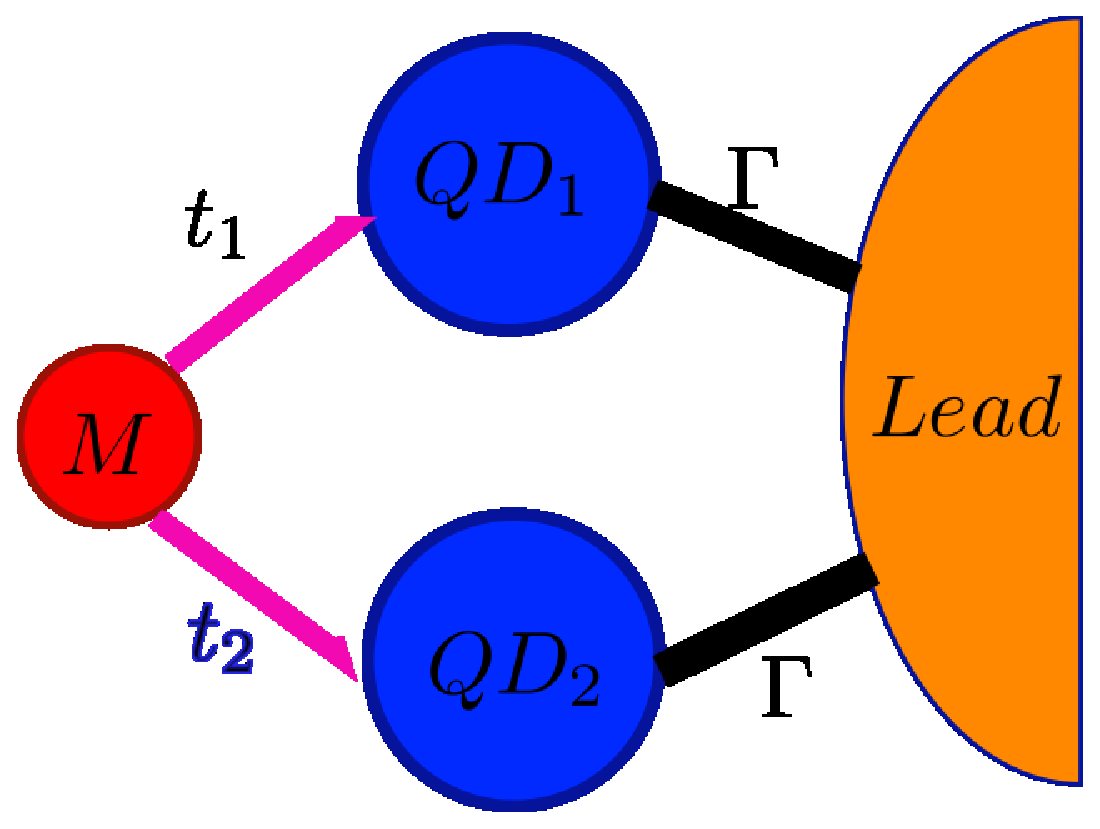
\includegraphics[scale=0.2]{Plots/Model/Majorana-2QD.eps}
% \caption{\label{fig:Mod/PHS-Shift_e2.png}$U_{1}=-2\ep_{d1}=0.5$, $\Gamma_{1}=\Gamma_{2}$,
% $t_{1}=t_2=0.02$. Variable $\ep_{d2} =\frac{U_{2}}{2}$}
% \end{figure*}
% \begin{figure}[hbt]
% \centering
% 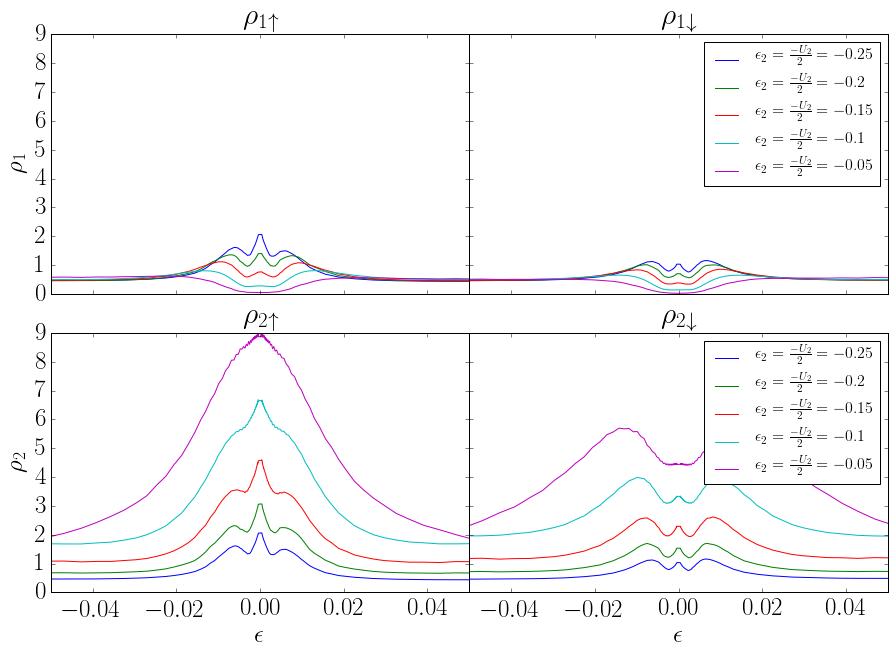
\includegraphics[scale=0.38]{Plots/DOS/PHS-Shift_e2.png}
% \caption{\label{fig:DOS/PHS-Shift_e2.png} Evolution of the QDs' DOS for the model in \ref{fig:Mod/PHS-Shift_e2.png} }
% \end{figure}
% We start again with the symmetric model with both QDs coupled to the Majorana mode, but this time the evolution is performed over $\ep_2=\frac{U}{2}$, such that the model is always Particle-Hole symmetric. This situation is very different from the previous model (\ref{sec:e2}) since the decaying of $U2$ 
% equalizes the effect of increasing the dot energy. In \ref{fig:DOS/PHS-Shift_e2.png} we observe that the DOS of QD2 increases while the QD1's DOS decreases, just as it happened in \ref{sec:e2} . However, the Majorana signature remains at $2$ for both dots , meaning that the Majorana is not preferably induced to tunnel to any QD despite the lose of symmetry in the dot energy.

% % \begin{figure}[hbt]
% % \centering
% % 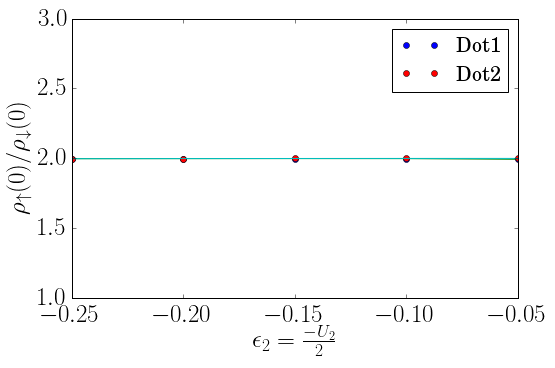
\includegraphics[scale=0.4]{Plots/MSig/PHS-Shift_e2.png}
% % \caption{\label{fig:MSig/PHS-Shift_e2} Relation between the spin up-down Zero-peaks at the Fermi level. The Majorana signature is related to $\frac{\rho_\up(0)}{\rho_\up(0)}=2$.}
% % \end{figure}

%---------------------------------------------------------------------------














% To built the ballistic transport graph (See \ref{sec:GraphMethod}) we just need to think that our model is actually merging the DQD graph (\ref{fig:graphDQD}) with the Majorana (Figure \ref{fig:green-M-QD}.b)). No need to write the green transport equations . Note  in graph $\MDQD$ that the  green function  $\Green{d_{1\downarrow},d_{1\downarrow}^{\dagger}}{\MDQD}$  is composed by the greeen function of the DQD $\left(\GreenG{d_{1\downarrow},d_{1\downarrow}^{\dagger}}{\GDQD } \right)$ and the extra term added by the presence of the majorana opperator $f_\downarrow$. In the equations this is simply 

% \begin{equation}
%     \GreenG{d_{1\downarrow},d_{1\downarrow}^{\dagger}}{\MDQD}=\left[\left(\GreenG{d_{1\downarrow},d_{1\downarrow}^{\dagger}}{\GDQD } \right)^{-1}+\frac{\omega}{\omega+\epsilon_{M}}\frac{E_{d_{1\dw}f_{\dw}}^{\MDQD}}{\left[\GreenG{f_{\downarrow},f_{\downarrow}^{\dagger}}{\MDQD-d_{1}}\right]^{-1}}\right]^{-1}.
% \end{equation}
% where 
% \begin{equation}
%     E_{d_{1\dw}f_{\dw}}^{\MDQD}=\left(t_{1}+t_{2}\frac{\left(t_{dots}+\sum_{\mathbf{k}}\frac{V_{1}V_{2}^{*}}{\omega-\epsilon_{\mathbf{k}}}\right)}{\omega-\epsilon_{2}-\sum_{\mathbf{k}}\frac{V_{2}V_{2}^{*}}{\omega-\epsilon_{\mathbf{k}}}}\right)\left(t_{1}^{*}+t_{2}^{*}\frac{\left(t_{dots}^{*}+\sum_{\mathbf{k}}\frac{V_{1}^{*}V_{2}}{\omega-\epsilon_{\mathbf{k}}}\right)}{\omega-\epsilon_{2}-\sum_{\mathbf{k}}\frac{V_{2}^{*}V_{2}}{\omega-\epsilon_{\mathbf{k}}}}\right).
% \end{equation}
% \Jesus{This fact is difficult to explain. I will need more plots and writing the appendix. For now I will leave here some results}

% We then need to compute $\GreenG{f_{\downarrow},f_{\downarrow}^{\dagger}}{\MDQD-d_{1}}$ . This graph is much simple. The neighborhood of  $f_{\downarrow}$ in graph ${\MDQD-d_{1}}$ are $d_2$ (above) and the inverted DQD(bellow). These neighbors are disconnected, hence we can include the in the green function independently. The term above is simply the dot $d_{2\downarrow}$ connected with the lead . 
% \begin{equation}
%     \frac{\frac{\omega}{\omega+\epsilon_{M}}\left\Vert t_{2}\right\Vert ^{2}}{\omega-\epsilon_{2}-\sum_{\mathbf{k}}\frac{V_{2}V_{2}^{*}}{\omega-\epsilon_{\mathbf{k}}}}.
% \end{equation}

 
% The term generated by the connection of $f_{\downarrow}$  with the inverted $DQD$ is a bit more complicated. First we need to include the term given by the connection with  $d_{2\downarrow}^\dagger$ which is 

% The other term is the contact with the DQD which can be expressed as 
% \begin{equation}
%     \GreenG{f_{\downarrow},f_{\downarrow}^{\dagger}}{\MDQD-d_{1}}=\left[\omega-\epsilon_{M}-\frac{\frac{\omega}{\omega+\epsilon_{M}}\left\Vert t_{2}\right\Vert ^{2}}{\omega-\epsilon_{2}-\sum_{\mathbf{k}}\frac{V_{2}V_{2}^{*}}{\omega-\epsilon_{\mathbf{k}}}}-\frac{\frac{\omega}{\omega+\epsilon_{M}}\left\Vert t_{2}\right\Vert ^{2}}{\omega+\epsilon_{2}-\sum_{\mathbf{k}}\frac{V_{2}V_{2}^{*}}{\omega+\epsilon_{\mathbf{k}}}}-\frac{\omega}{\omega+\epsilon_{M}}\frac{E_{f_{\dw}d_{1\dw}^\dagger}^{\MDQD-d_1}}{\left[\GreenG{d_{1\downarrow}^{\dagger},d_{1\downarrow}{\dagger}}{\MDQD-d_{1}-f_{\downarrow}}\right]^{-1}}\right]^{-1}.
% \end{equation}
% Now, note that that graph $\MDQD-d_{1}-f_{\downarrow}$ is actually a double quantum dot with negated couplings. Hence  $\GreenG{d_{1\downarrow}^{\dagger},d_{1\downarrow}{\dagger}}{\MDQD-d_{1}-f_{\downarrow}}$  satisfies the equation \eqref{eq:solGreen} but with variables $-t_{dots}, -t_1 , -t_2, -\ed{1}  , -\ed{2}$



